\PassOptionsToPackage{hidelinks}{hyperref}

\documentclass[jou,12pt,floatsintext]{apa7} % man doc stu jou


% 语言和字体设置
\usepackage[american]{babel}
\usepackage{ctex}
\usepackage{xeCJK}
\setCJKmainfont{Songti SC Regular} % 设置中文主字体为 STSong,字间距增加
\setmainfont{Times New Roman} % 设置英文字体

\setlength\parindent{2em}

% 参考文献设置
\usepackage{csquotes}
\usepackage[style=apa,sortcites=true,sorting=nyt,backend=biber]{biblatex}
\DeclareLanguageMapping{american}{american-apa}
\addbibresource{bibliography.bib}

%绘图用
\usepackage{caption}
\usepackage{graphicx}
\usepackage{float} 
\usepackage{subcaption}
% \usepackage{subfigure}





% Title page stuff _____________________
\title{\heiti 语言和音乐的调制频率} % The big, long version of the title for the title page
\shorttitle{APA Starter} % The short title for the header
\author{\fangsong 毛沛炫}
\duedate{April 20, 2024}
% \date{January 17, 2024} The student version doesn't use the \date command, for whatever reason
\affiliation{(浙江大学心理与行为科学系\ \ 310058)}
\course{PSY 4321} % LaTeX gets annoyed (i.e., throws a grumble-error) if this is blank, so I put something here. However, if your instructor will mark you off for this being on the title page, you can leave this entry blank (delete the PSY 4321, but leave the command), and just make peace with the error that will happen. It won't break the document.
\professor{Dr. Professor}  % Same situation as for the course info. Some instructors want this, some absolutely don't and will take off points. So do what you gotta.

\usepackage{changepage}


\abstract{该实验通过分析个人录制的音频样本,探讨语音和音乐在调制频率上的差异,并探索特定发声动作(弹舌)的调制频率。结果显示,普通话阅读的调制频率峰值为4.8Hz,而歌唱约为1.5Hz,证实了语音和音乐在主调制频率上的显著差异,与大规模语料库研究结果一致。此外,弹舌产生了约27.3Hz的高频调制峰值,方言的调制峰值(约6Hz)略高于普通话阅读。本研究结果支持语音和音乐调制频率存在固有差异的观点,并指出唱歌的调制频谱在20-30Hz频段存在一个较为明显的波峰。\\
\textbf{\heiti 关键词}\ \ \ \ 调制频率,语音,音乐,弹舌,方言}


% Set up fancy header/footer
\usepackage{fancyhdr}
\pagestyle{fancy}
\fancyhead[LO,L]{\thepage}
\fancyhead[CO,C]{信号与认知系统}
\fancyhead[RO,R]{}
% % \fancyfoot[LO,L]{}
% % \fancyfoot[CO,C]{\thepage}
% % \fancyfoot[RO,R]{}
% \renewcommand{\headrulewidth}{0.4pt}
% % \renewcommand{\footrulewidth}{0.4pt}


% \keywords{哈哈哈,啊上岛咖啡} % If you need to have keywords for your paper, delete the % at the start of this line


\begin{document}

\begin{titlepage}
    \centering
    \vspace*{4cm} % 调整标题的垂直位置
    \Huge
    {\heiti 语言和音乐的调制频率} \\
    \vspace{0.75cm}
    \large
    信号与认知系统 \\
    \vspace{2.25cm}
    % \vspace{2cm}
    \large
    毛沛炫\ \ \ 3220102692 \\
    \vspace{0.5cm}
    \large
    心理与行为科学系 \\
    \vspace{0.5cm}
    \large
    \number\year 年 \number\month 月 \number\day 日 \\
    % \vspace{12.3cm}
    % \today
    % \number\year 年 \number\month 月 \number\day 日
    \vfill
\end{titlepage}

\maketitle % This tells LaTeX to make the title page



% Since the Introduction is where references in papers first show up, let us incorporate some now. There are some intricacies to be aware of when using \LaTeX{} to write your paper (yes, there is a \LaTeX{} command to make it look fancy like that, because of course there is). Referencing something \textbf{in text} is done by dropping the name in text with the year followed in parentheses; lucky for us \LaTeX{} handles it with the right command, like  \textcite{Sample2024}. But maybe you want to just include it all at as a \textbf{parenthetical}? \LaTeX{} can do that as well \parencite{FullBook2021}. %For multi-author works \parencite[e.g.,]{Multiauthor2020}, the full author list will be included the first time. However, on subsequent reappearances of that reference, it will be shortened as APA intended \parencite{Multiauthor2020}.
% For whatever reason, it does not seem like the multi-author work \parencite[e.g.,][]{Multiauthor2020} is working as it should, where it gives the full list the first time it is included in text, then truncates afterwards \parencite{Multiauthor2020}. I am not sure what is up with that, so the best advice I can offer you is to do write out the first instance yourself, then let \LaTeX{} handle the rest. It sucks, I know. Such is the nature of the \LaTeX{} beast, sometimes.

\section{引言}

\subsection{\heiti 研究背景}
语音和音乐是人类两种基本的声音交流形式,它们都具有复杂的节奏结构。尽管人们可以在感知上轻易的区分开语言交流和音乐,但本质上它们都属于声音信号,其声音强度随时间发生波动,即受到时间调制(temporal modulations)。理解语音和音乐中的时间调制特性,对于揭示人类听觉系统处理复杂声音的机制至关重要。

在语音和音乐中的时间调制特性的研究中,调制谱(modulation spectrum)分析已成为一种重要的研究工具。调制谱能够量化声音信号中不同调制频率的强度,揭示声音信号的节奏特征。早期的研究表明,语音和音乐的调制谱都具有1/f的特征\parencite{voss1975,mozer1996,decoensel2003,singh2003modulation},但也有研究指出语音的调制谱在4-5 Hz附近存在峰值\parencite{houtgast1985review,chi1999spectro,greenberg1999speaking,greenberg2003temporal,goswami2013speech}。这些不一致的结果促使研究者们对语音和音乐的调制谱进行更深入的探索。

过往研究结果结论不同,或许是因为不同研究者采取的数据处理方法不同。为了寻求一个更加普遍而又简洁的规律,\textcite{ding2017temporal}对语言和音乐使用了一致的分析方法,对9种语言(共超过25小时)的语音数据和多种西方音乐风格(共超过39小时)的音乐数据进行了调制谱分析。研究结果表明:语音调制谱具有高度一致性:尽管不同语言在韵律上存在差异,但它们的语音调制谱都表现出显著的相似性,峰值频率集中在4-5Hz;音乐调制谱与语音明显不同,音乐的调制谱峰值频率明显低于语音,主要集中在2Hz以下;语音的调制峰值频率与音节率密切相关,而音乐的调制峰值频率则与节拍(beat)频率及其倍频相关。

\subsection{\heiti 研究目的}

本实验旨在通过简单的材料复现\textcite{ding2017temporal}的部分研究结果,主要通过以下两个方面进行实验:(1)个人语音和音乐的调制谱分析: 我们将录制自己说一段话和唱一段歌的音频,并分析其调制谱,与文献中的结果进行比较,验证语音和音乐调制谱的差异性;(2)探索快速调制频率的极限:我们将尝试通过不同的身体运动(如敲击、走路、说话)来产生声音,并分析其调制谱,探索人类在非言语/音乐情境下能够通过运动产生的最快调制频率。


\section{方法}


\subsection{\heiti 实验材料}

一段使用普通话(Mandarin)阅读书本的录音,时长38秒;一段使用普通话演唱的歌曲(song),无伴奏,时长53秒;一段实验者和母亲通过方言(dialect)交流的录音,时长46秒;一段通过身体运动产生的声音,时长26秒。所有录音都通过实验者的个人手机的系统录音机获取,采样率均为48kHz。
在本实验中,实验者采用的身体运动方式为弹舌(tongue trill),又称齿龈颤音。弹舌的调音方法是用舌尖抵住上齿龈脊进行调音,是一种通过快速震动舌头产生的声音,是一种常见的音乐技巧,也是一种辅音,常见于俄语、西班牙语等。实验者通过快速震动舌头,产生一种类似``rrrrr''(或类似于``tttttt'')的声音。

\subsection{\heiti 数据处理}

为量化音频信号中的时间调制特性,实验对录制的语音、歌唱及运动产生的声音片段进行了调制谱分析\parencite{ding2017temporal}。为了模拟人耳外周听觉系统的处理过程,信号通过一个耳蜗模型进行滤波,该模型将声音信号分解为多个不同中心频率的窄带信号,模拟耳蜗不同位置对不同频率声音的响应。耳蜗模型输出为音频信号的时频图(spectrogram),反映了不同频带的声音信号强度随时间的变化。接着,通过平方提取每个窄带通道的瞬时功率包络。核心的调制谱计算涉及对每个通道的时间包络应用离散傅里叶变换(Discrete Fourier Transform, DFT),将其从时域转换到调制频域。计算每个DFT系数的绝对值后,通过计算所有窄带通道幅度谱的均方根(Root Mean square, RMS)平均值,得到该音频片段最终的调制谱。整个数据处理流程均采用\textcite{ding2017temporal}提供的MATLAB工具箱进行。

\section{结果}

\subsection{\heiti 说话和唱歌的调制谱分析}

\begin{figure*}[!htb]
    \centering
    % 第一行子图
    \begin{minipage}{0.49\textwidth}
        \centering
        \subcaption{}
        \vspace{-0.5em}
        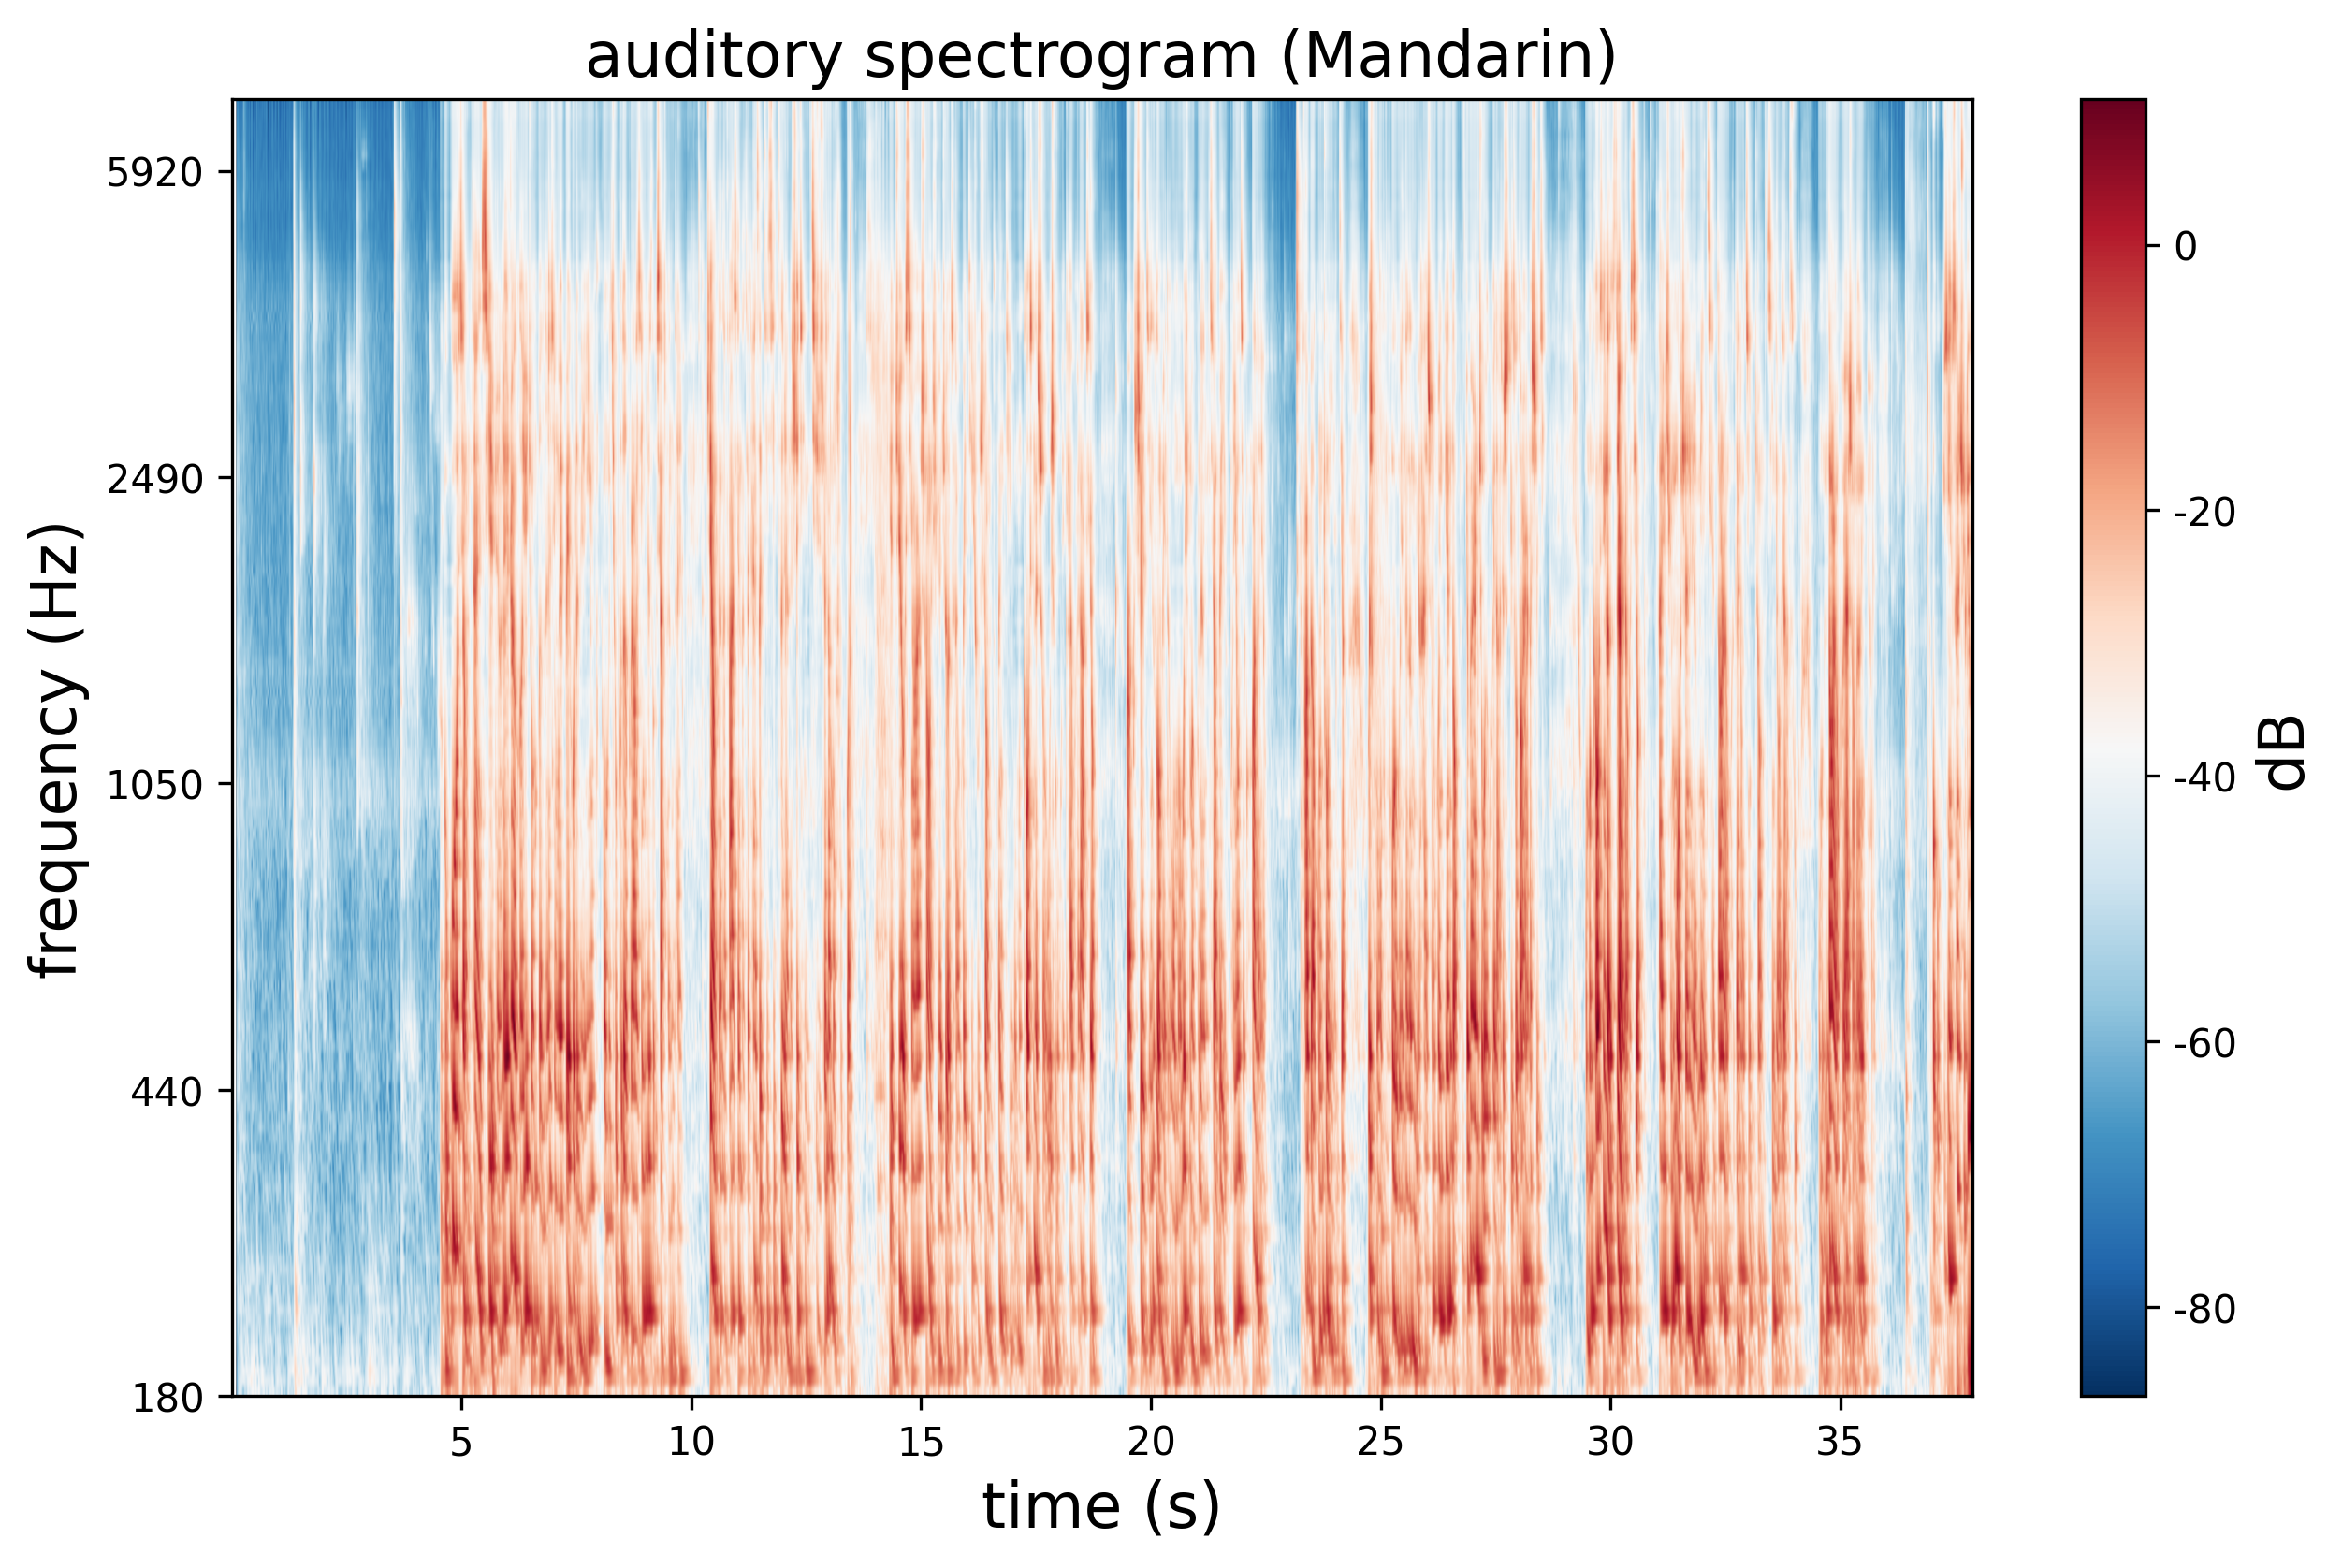
\includegraphics[width=\textwidth]{figure/shuohua.png}
        \label{spectrogram:shuohua}
    \end{minipage}
    \begin{minipage}{0.49\textwidth}
        \centering
        \subcaption{}
        \vspace{-0.5em}
        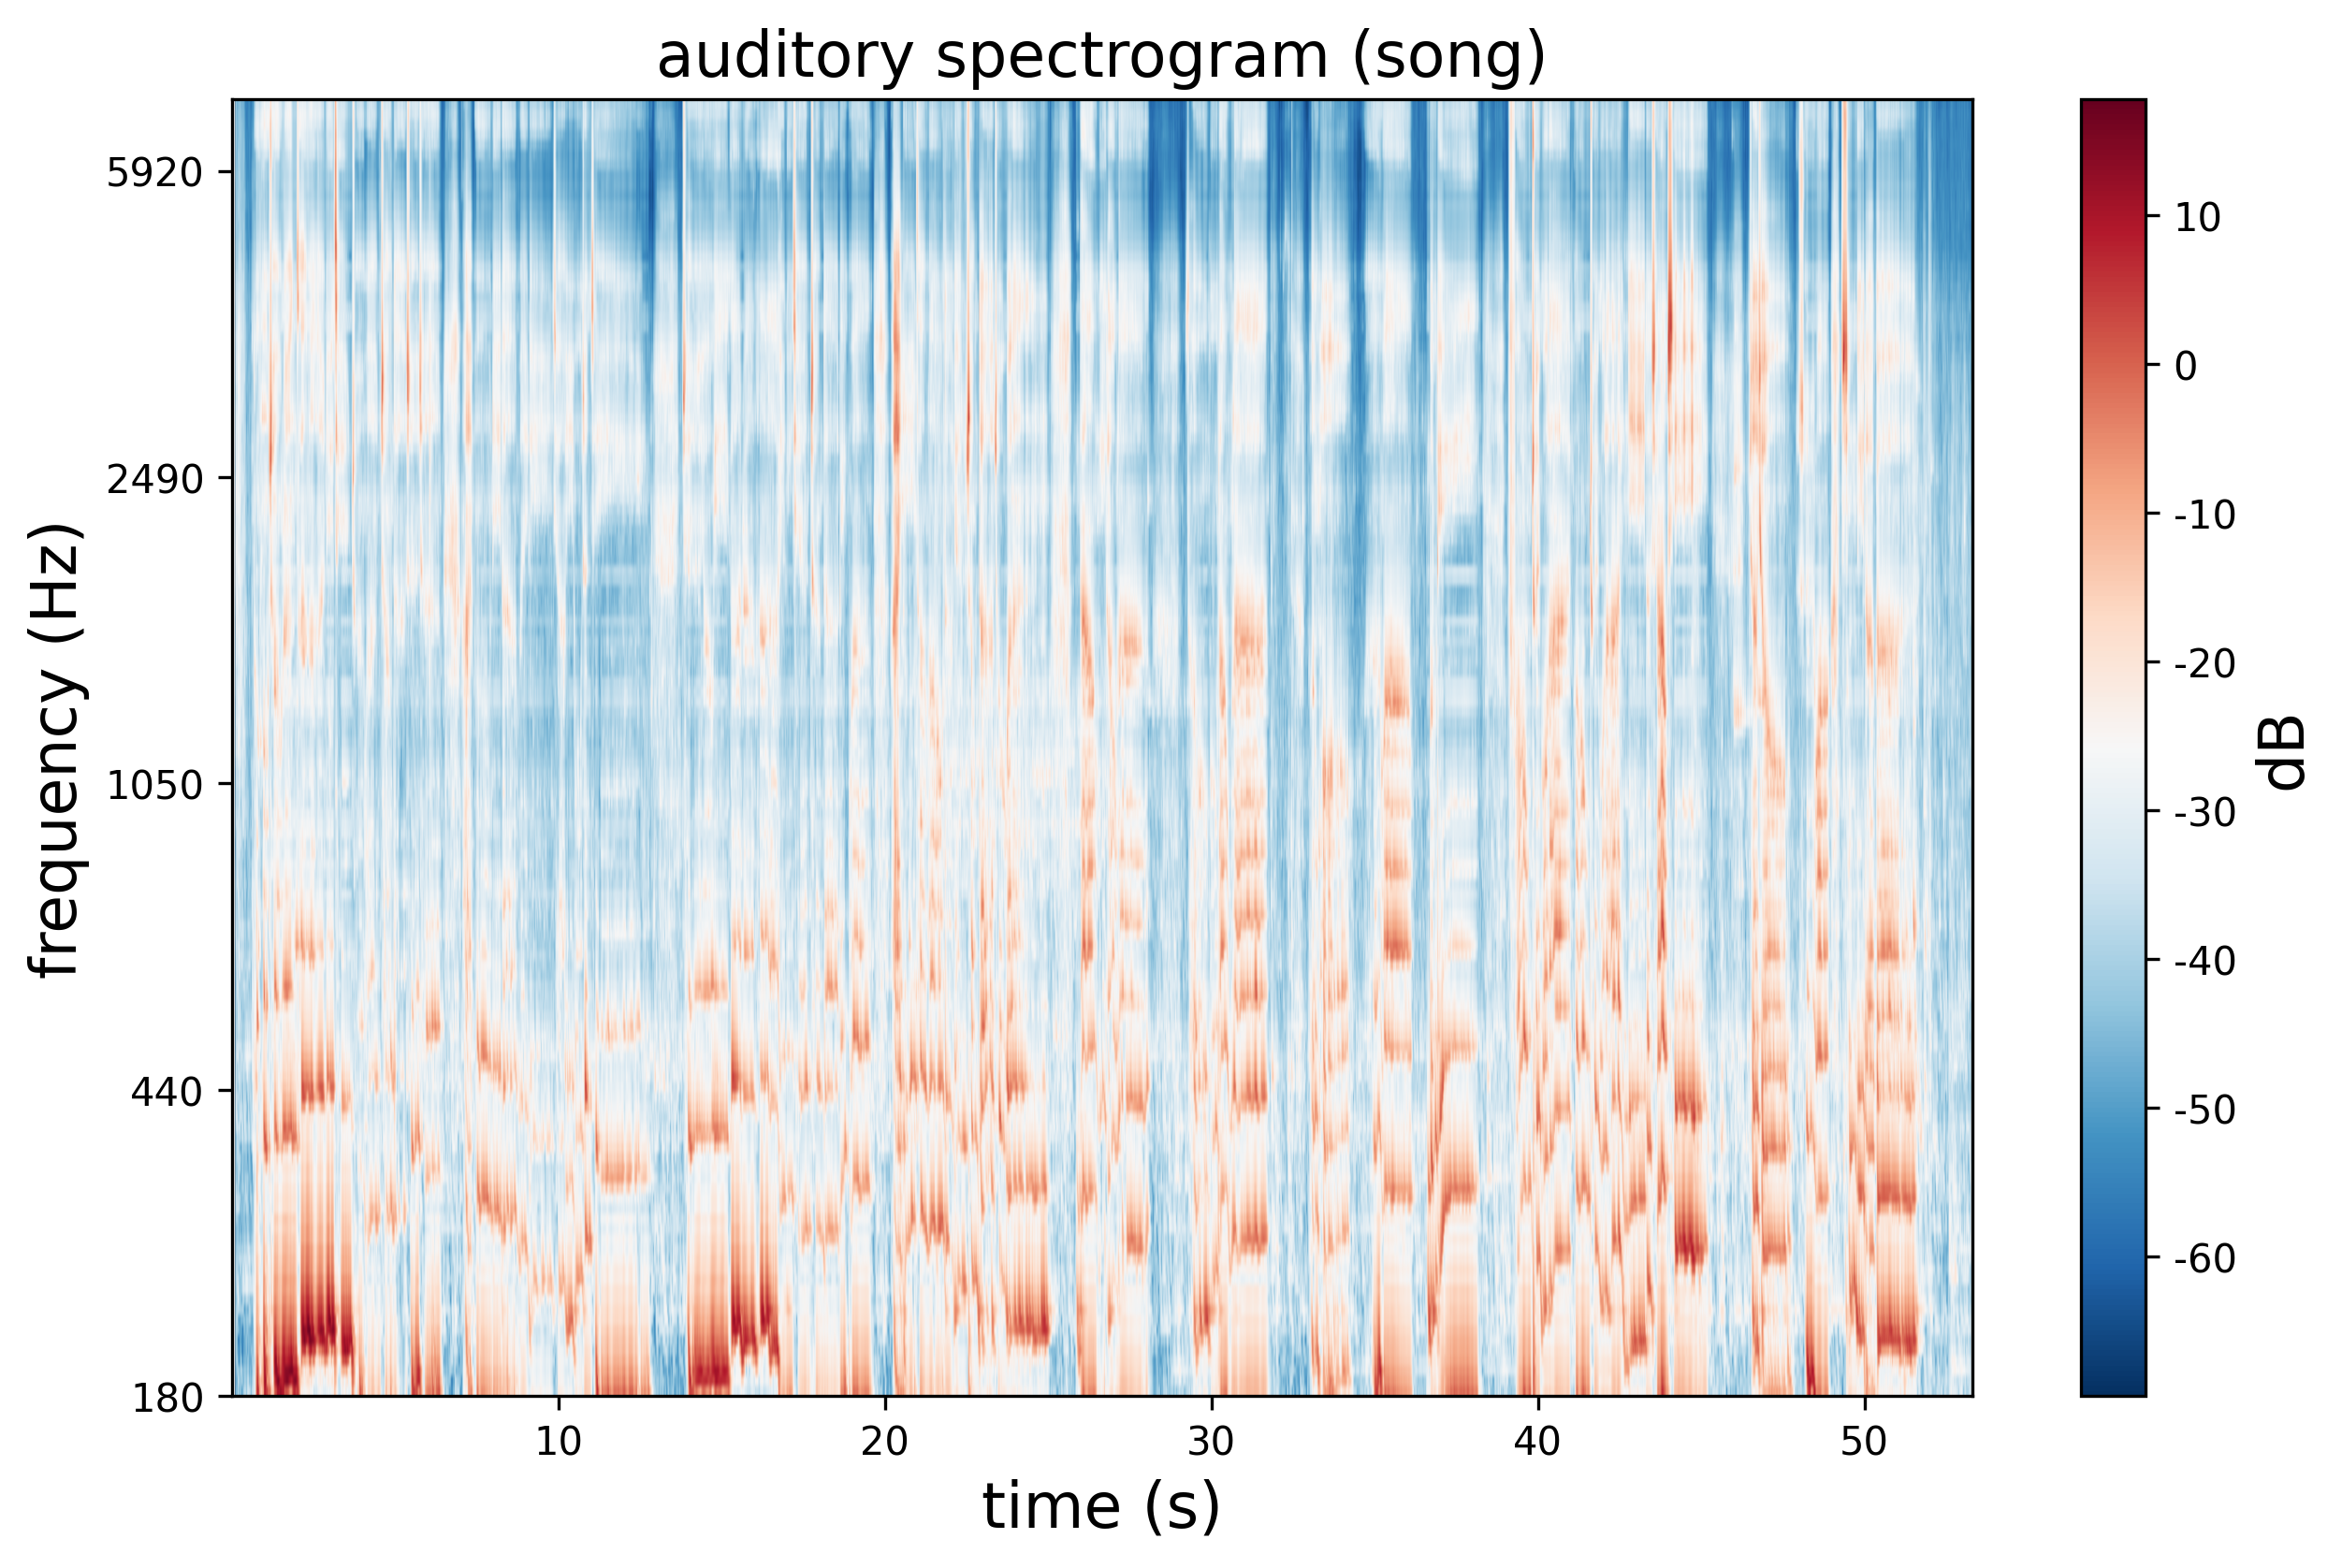
\includegraphics[width=\textwidth]{figure/song.png}
        \label{spectrogram:song}
    \end{minipage}
    
    \vspace{-2em} % 调整两行子图之间的间距
    
    % 第二行子图
    \begin{minipage}{0.49\textwidth}
        \centering
        \subcaption{}
        \vspace{-0.5em}
        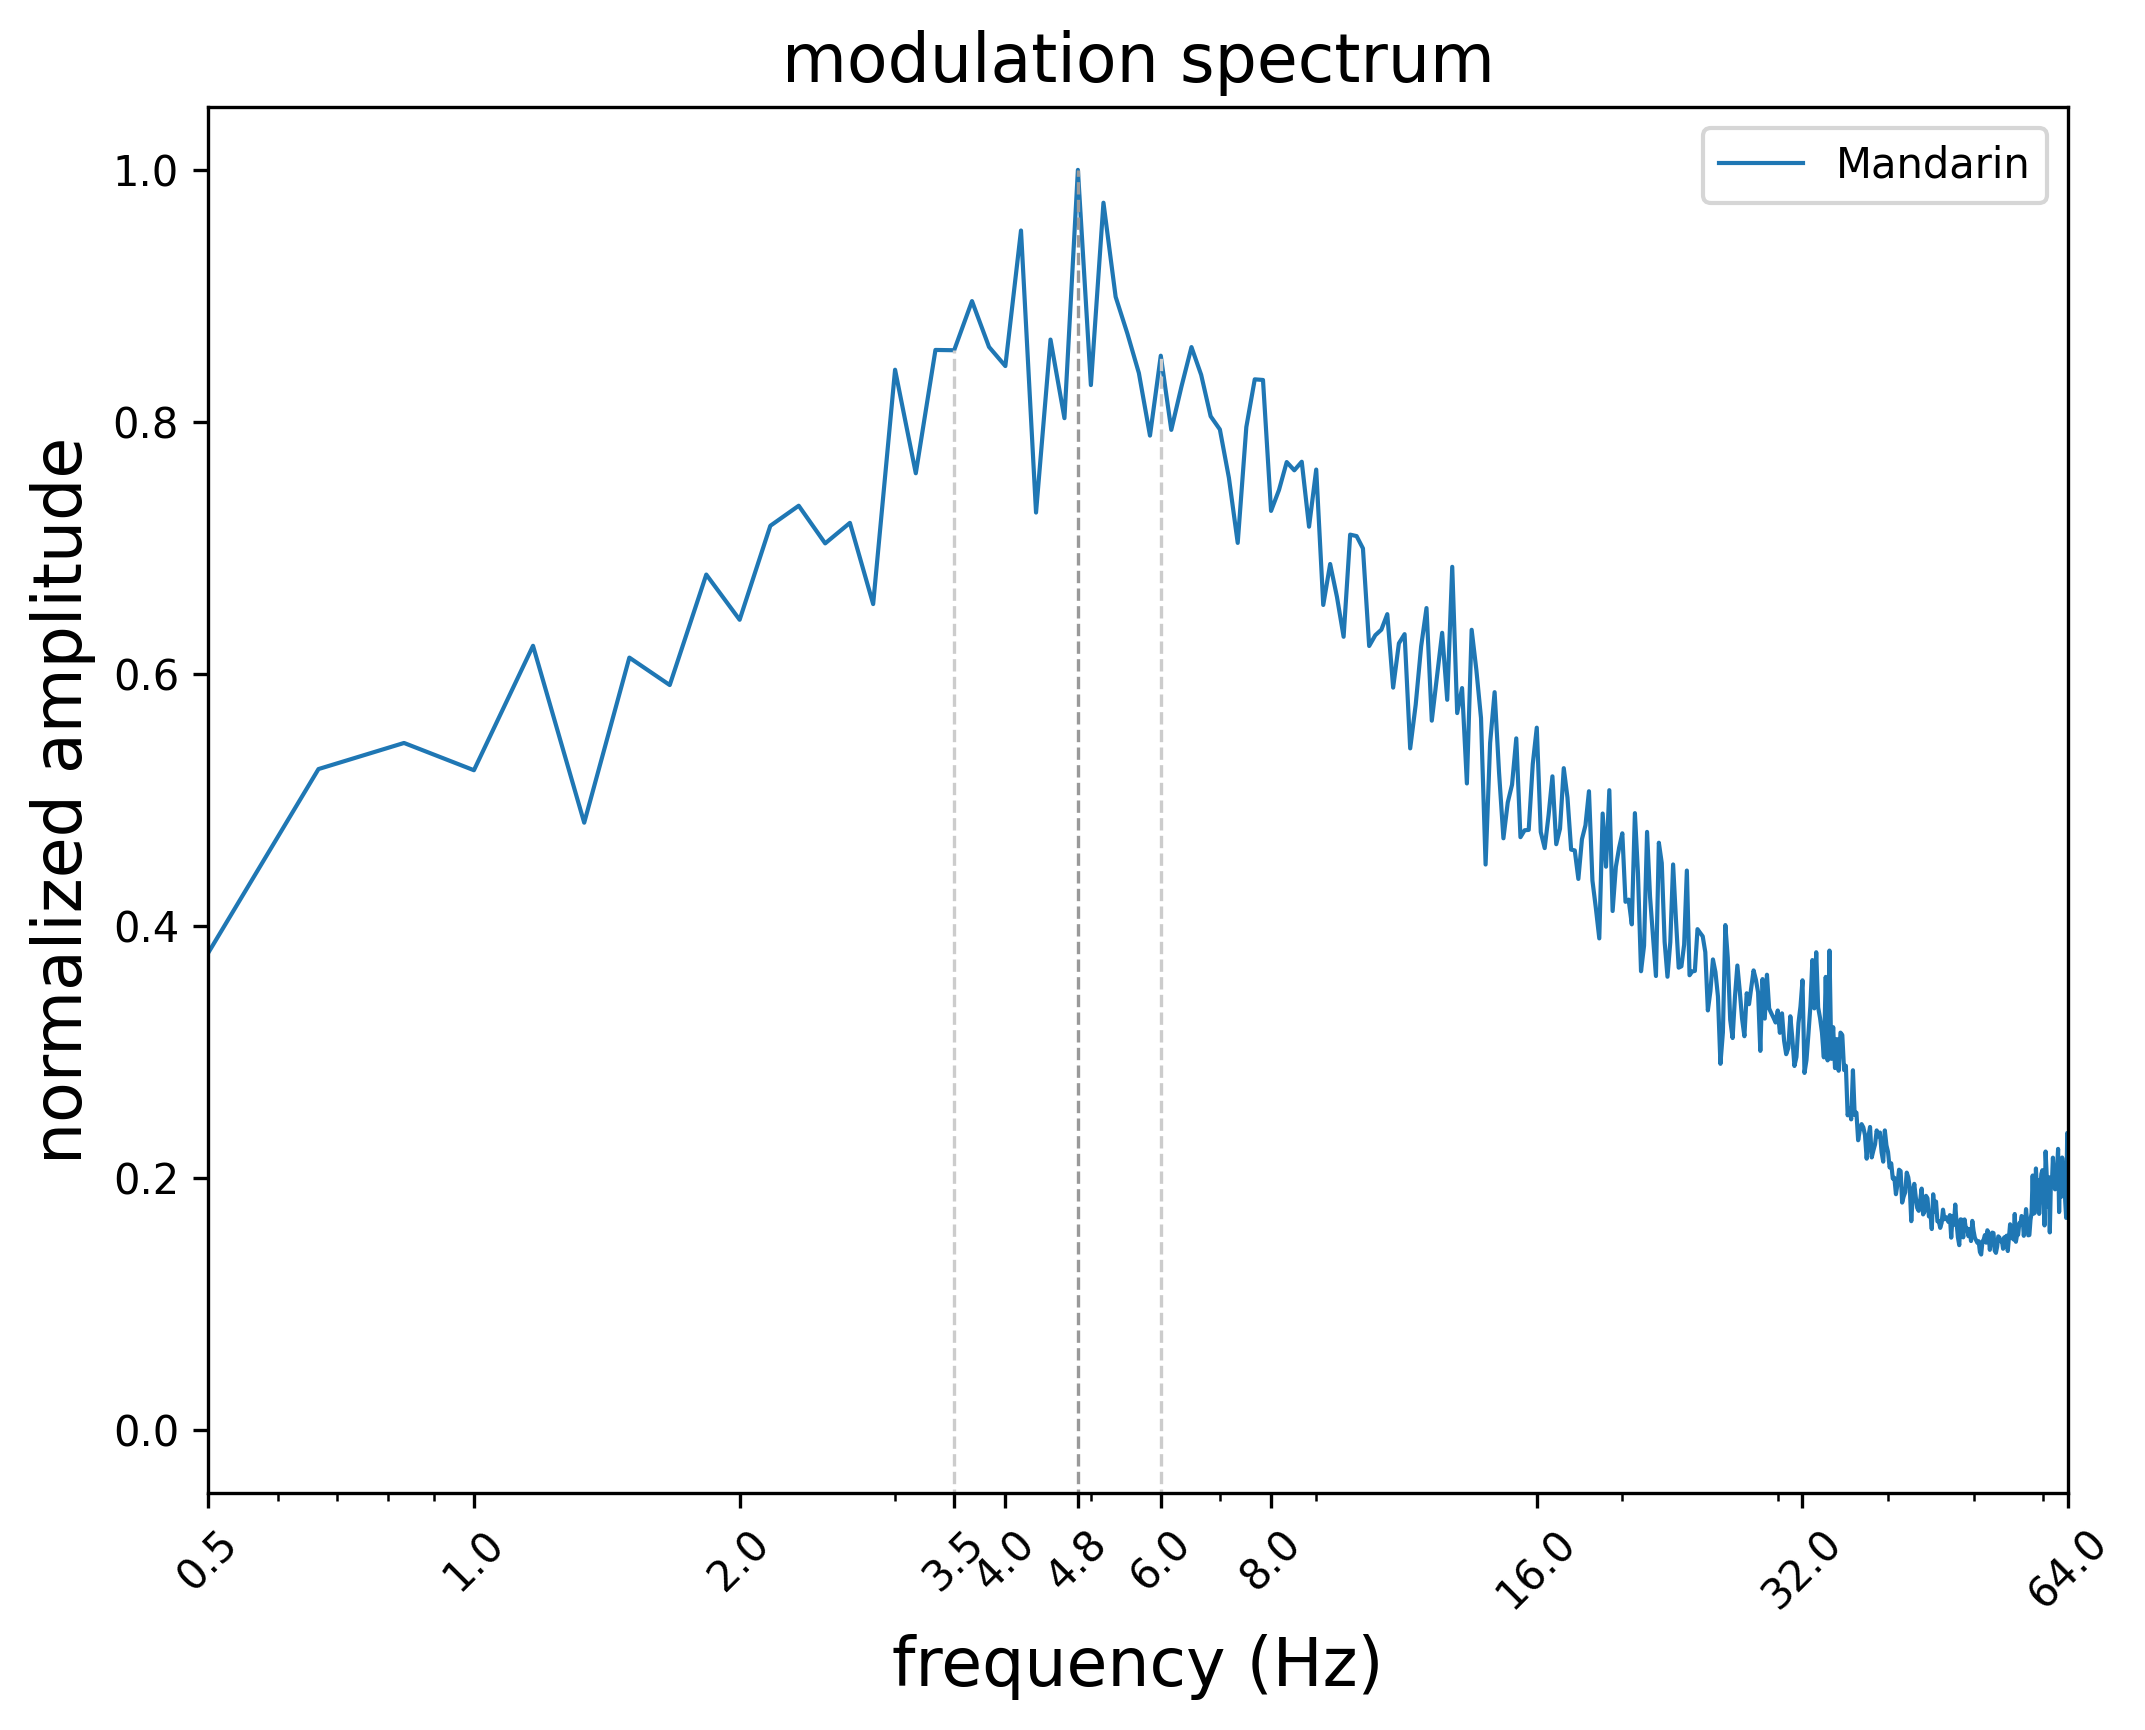
\includegraphics[width=\textwidth]{figure/spectrum_shuohua.png}
        \label{spectrum:shuohua}
    \end{minipage}
    \begin{minipage}{0.49\textwidth}
        \centering
        \subcaption{}
        \vspace{-0.5em}
        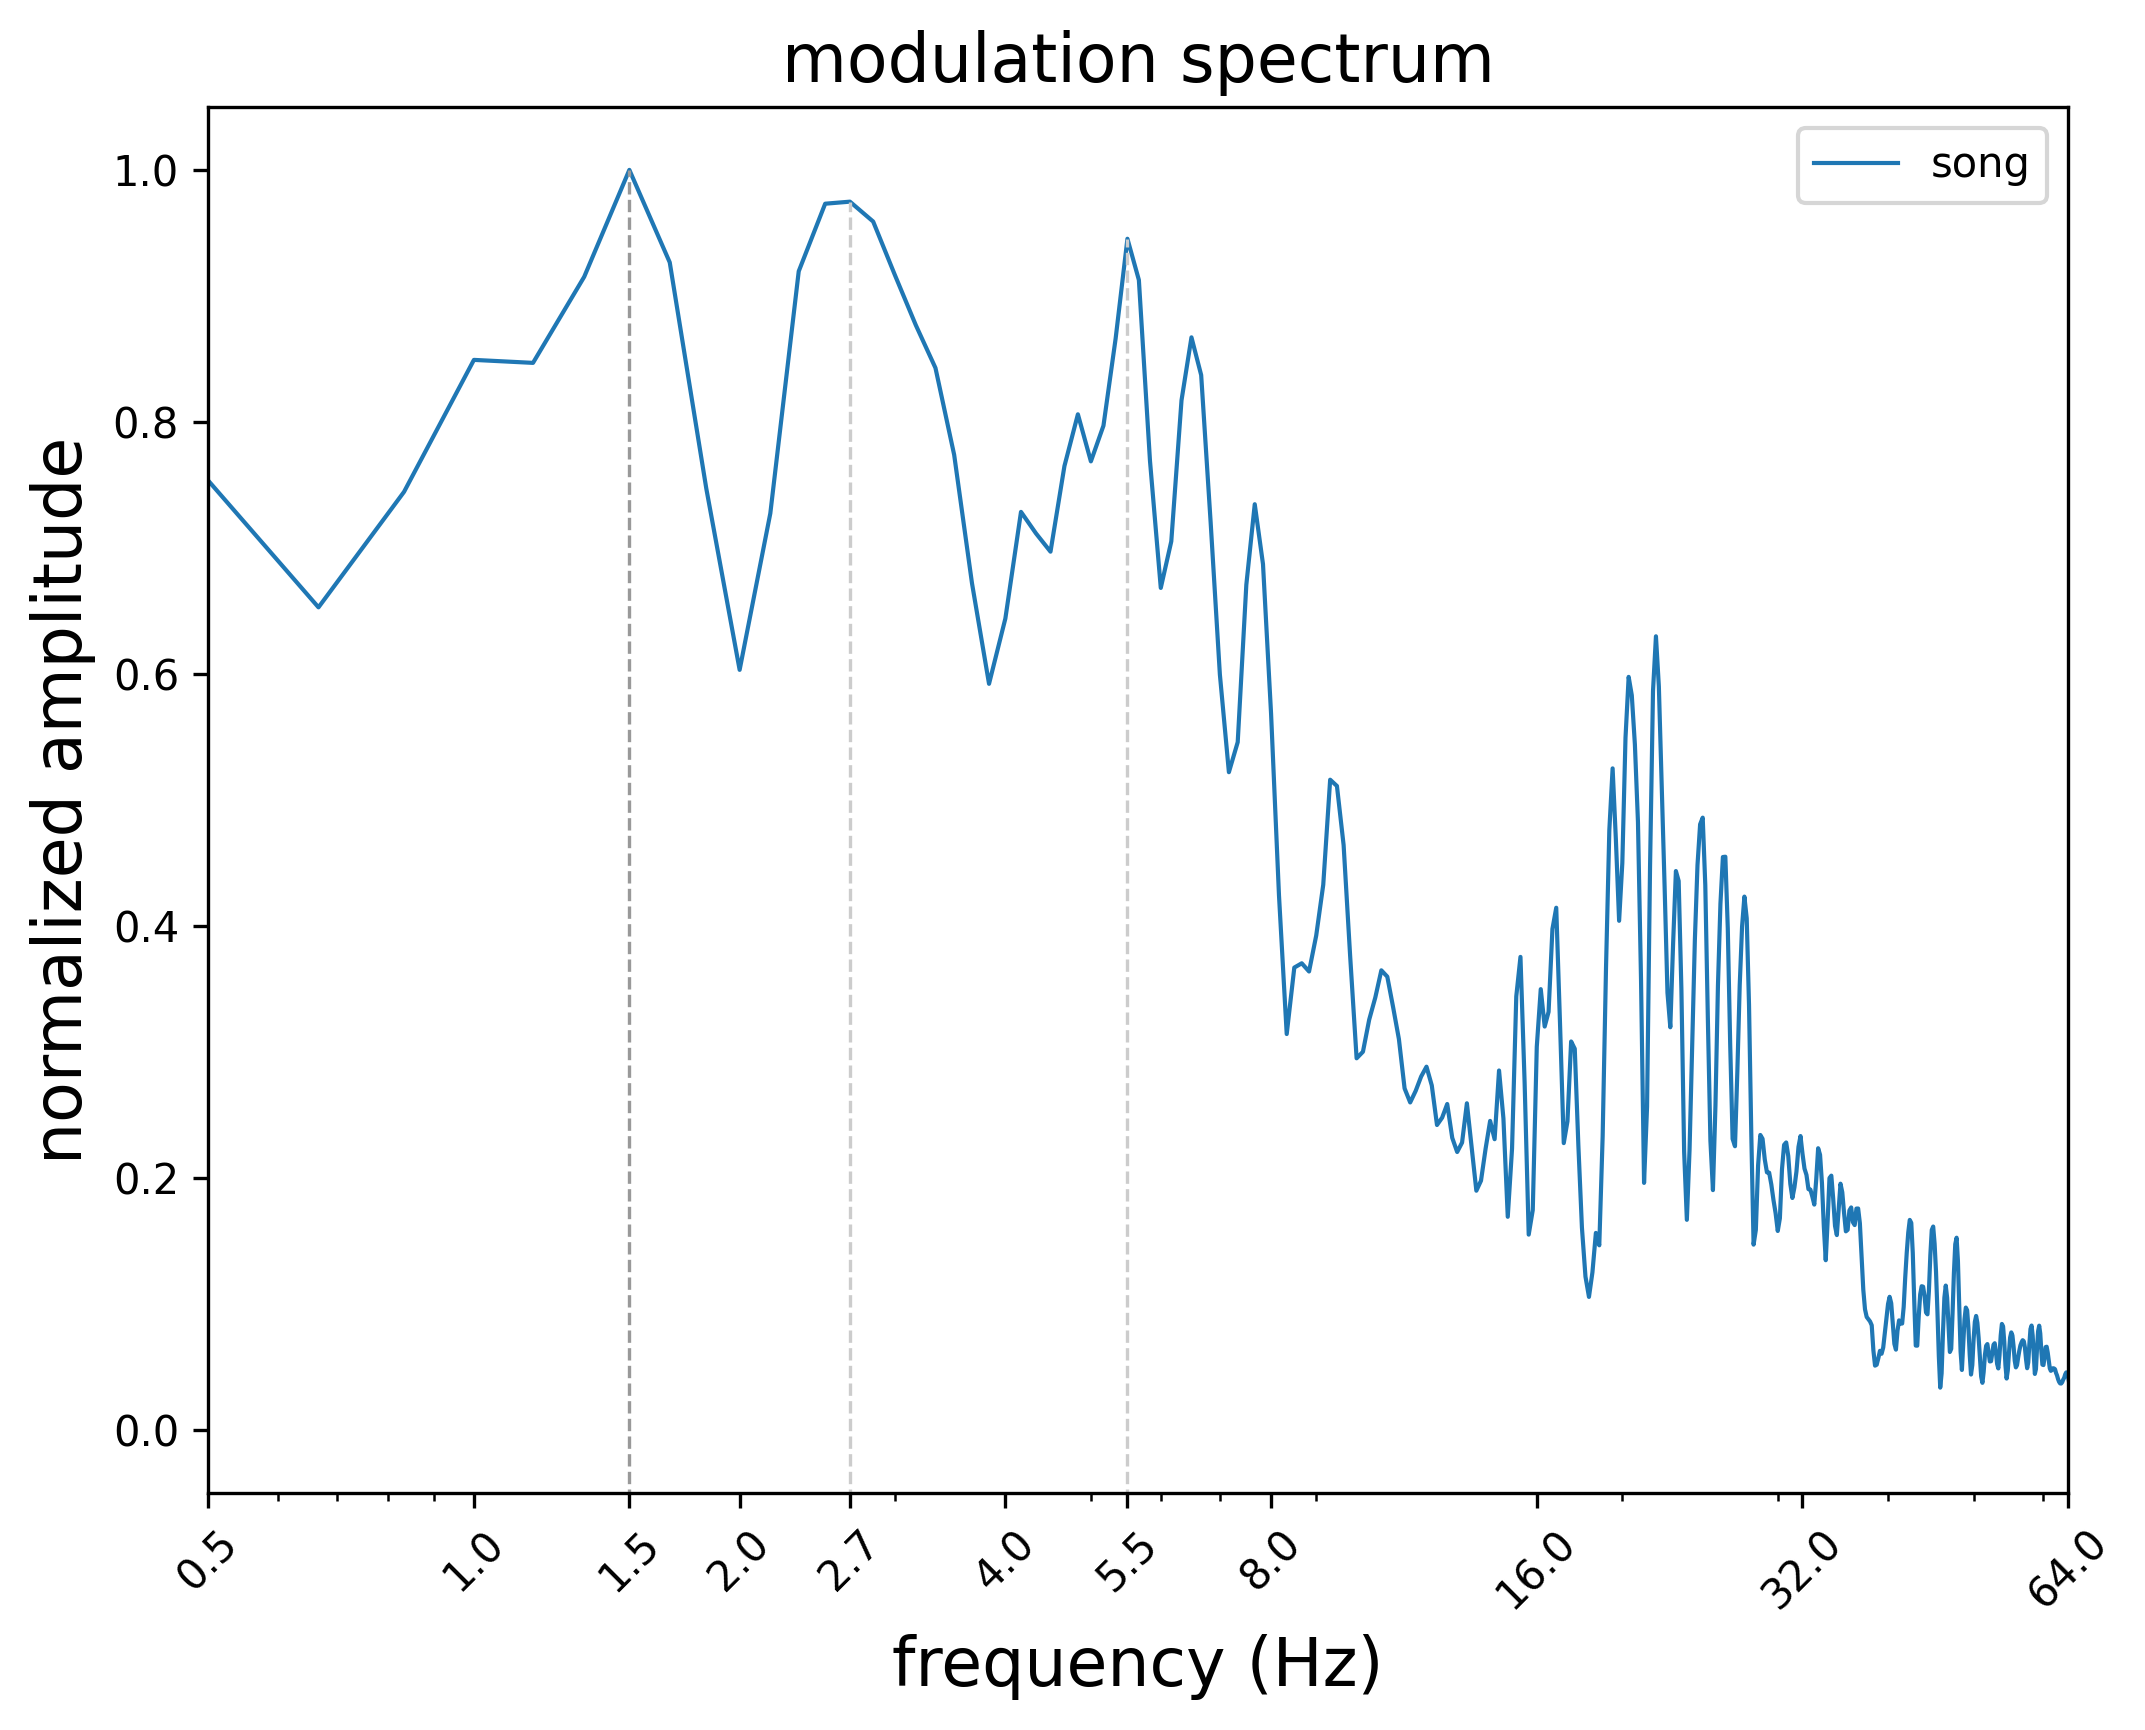
\includegraphics[width=\textwidth]{figure/spectrum_song.png}
        \label{spectrum:song}
    \end{minipage}
    
    \captionsetup{labelsep=period}
    \vspace{-1em}
    \caption{\small 个人普通话语音和歌唱的时频图和调制谱}
    
    \label{fig:fig1}
\end{figure*}

普通话阅读书本、唱歌的时频分析见图\ref{spectrogram:shuohua}和\ref{spectrogram:song},调制谱分析见\ref{spectrum:shuohua}和\ref{spectrum:song}。从时频分析图可以直观地看出,阅读时的音调和音强基本保持恒定;而唱歌时的音调则随着旋律的变化而不断改变,且不同歌词之间的音强也有细微的差异。调制谱分析表明,实验者阅读的调制频率主要在3.5-6.0Hz之间,4.8Hz是最主要的调制频率;唱歌的调制谱在频域上有一个较宽的波峰(1-6Hz),在1.5Hz、2.7Hz、5.5Hz处各存在一个峰值,其中1.5Hz为最主要的调制频率,且在20-30Hz之间还有一个小波峰。

可以看出,人唱歌的最主要的调制频率(1.5Hz)明显小于阅读(4.8Hz)。实验者清唱的歌曲为88bpm,八六拍,因此音乐最主要的调制频率应该是1.467Hz(即88/60),和最主要的调制频率1.5Hz接近。此外,调制谱中2.7Hz、5.5Hz处的峰值也大约等于1.467Hz的2倍和4倍,和之前的研究结果一致\parencite{ding2017temporal}。

唱歌的调制谱在20-30Hz之间还有一个小波峰,这和\textcite{ding2017temporal}研究中的中提琴(viola)的调制谱非常相似。两者调制谱的相似是可以预见的,因为中提琴是之前研究中频率和人声最为接近的乐器(最接近的是大提琴,但是之前研究并未分析大提琴的调制谱)。然而,至于为什么唱歌和中提琴的调制谱在20-30Hz之间有一个明显的小波峰,这个问题还有待进一步研究。

\begin{figure*}[!htb]
    \centering
    % 第一行子图
    \begin{minipage}{0.49\textwidth}
        \centering
        \subcaption{}
        \vspace{-0.5em}
        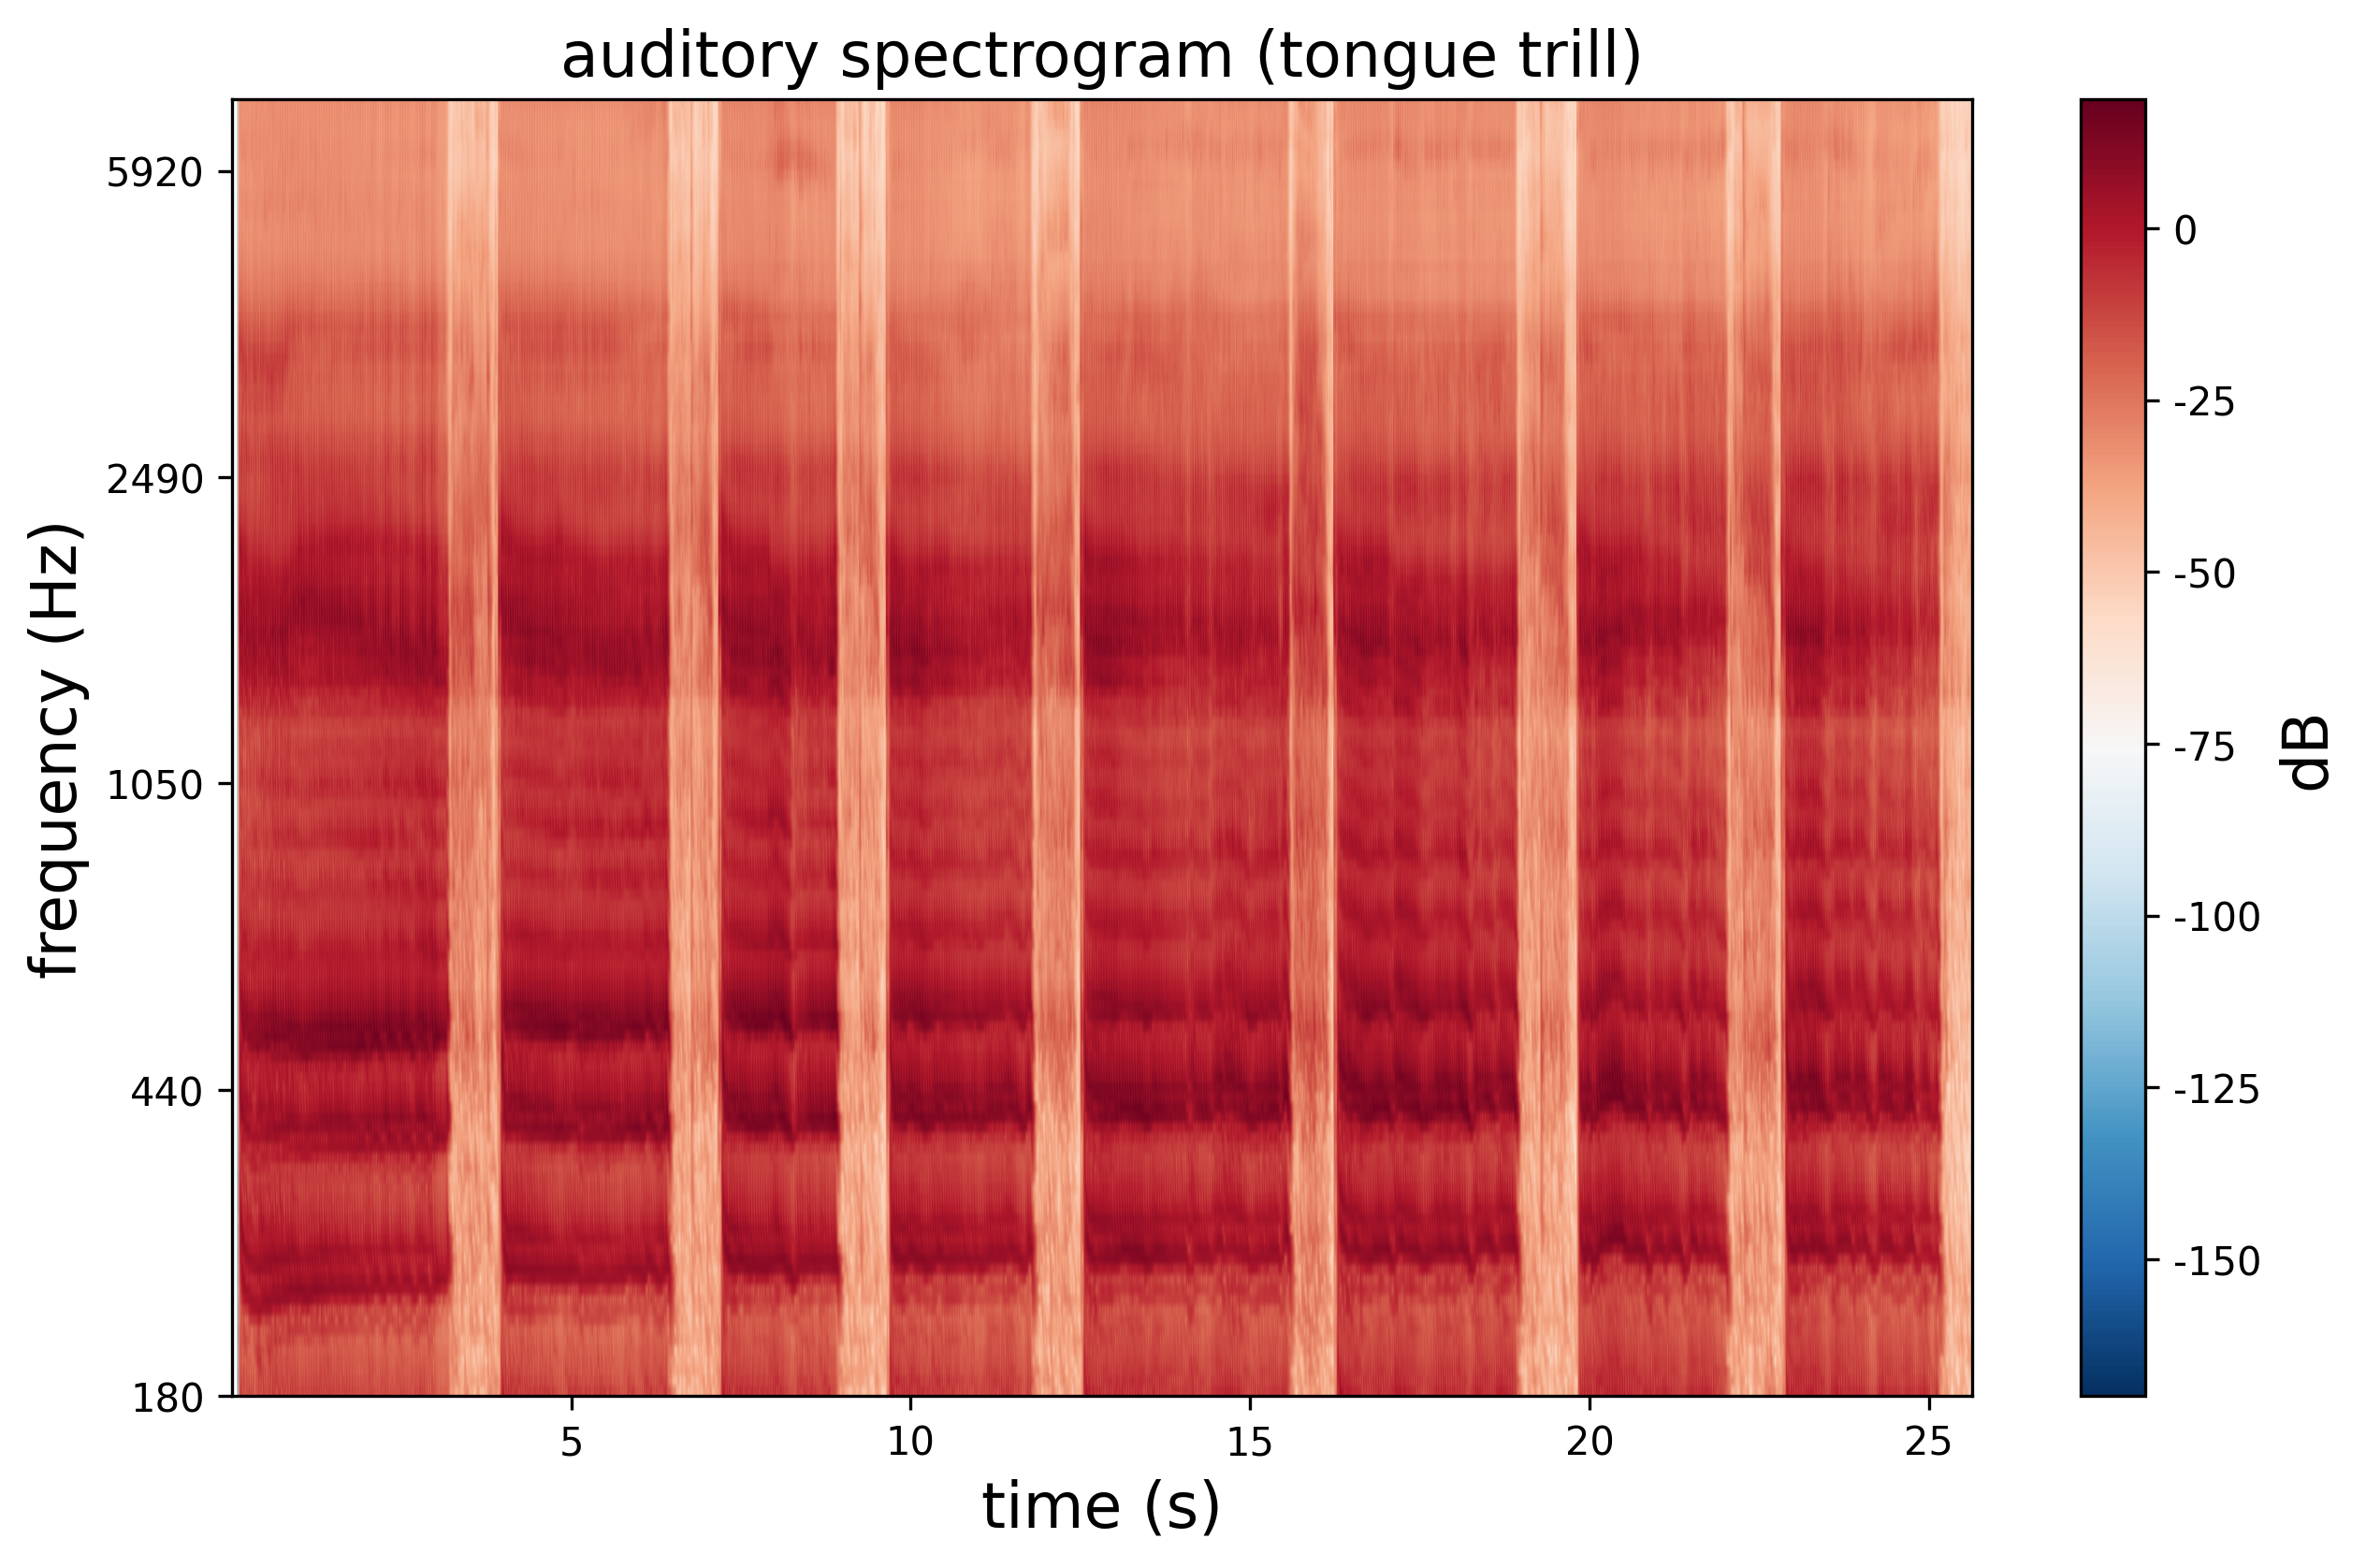
\includegraphics[width=\textwidth]{figure/tanshe.png}
        \label{spectrogram:tanshe}
    \end{minipage}
    \begin{minipage}{0.49\textwidth}
        \centering
        \subcaption{}
        \vspace{-0.5em}
        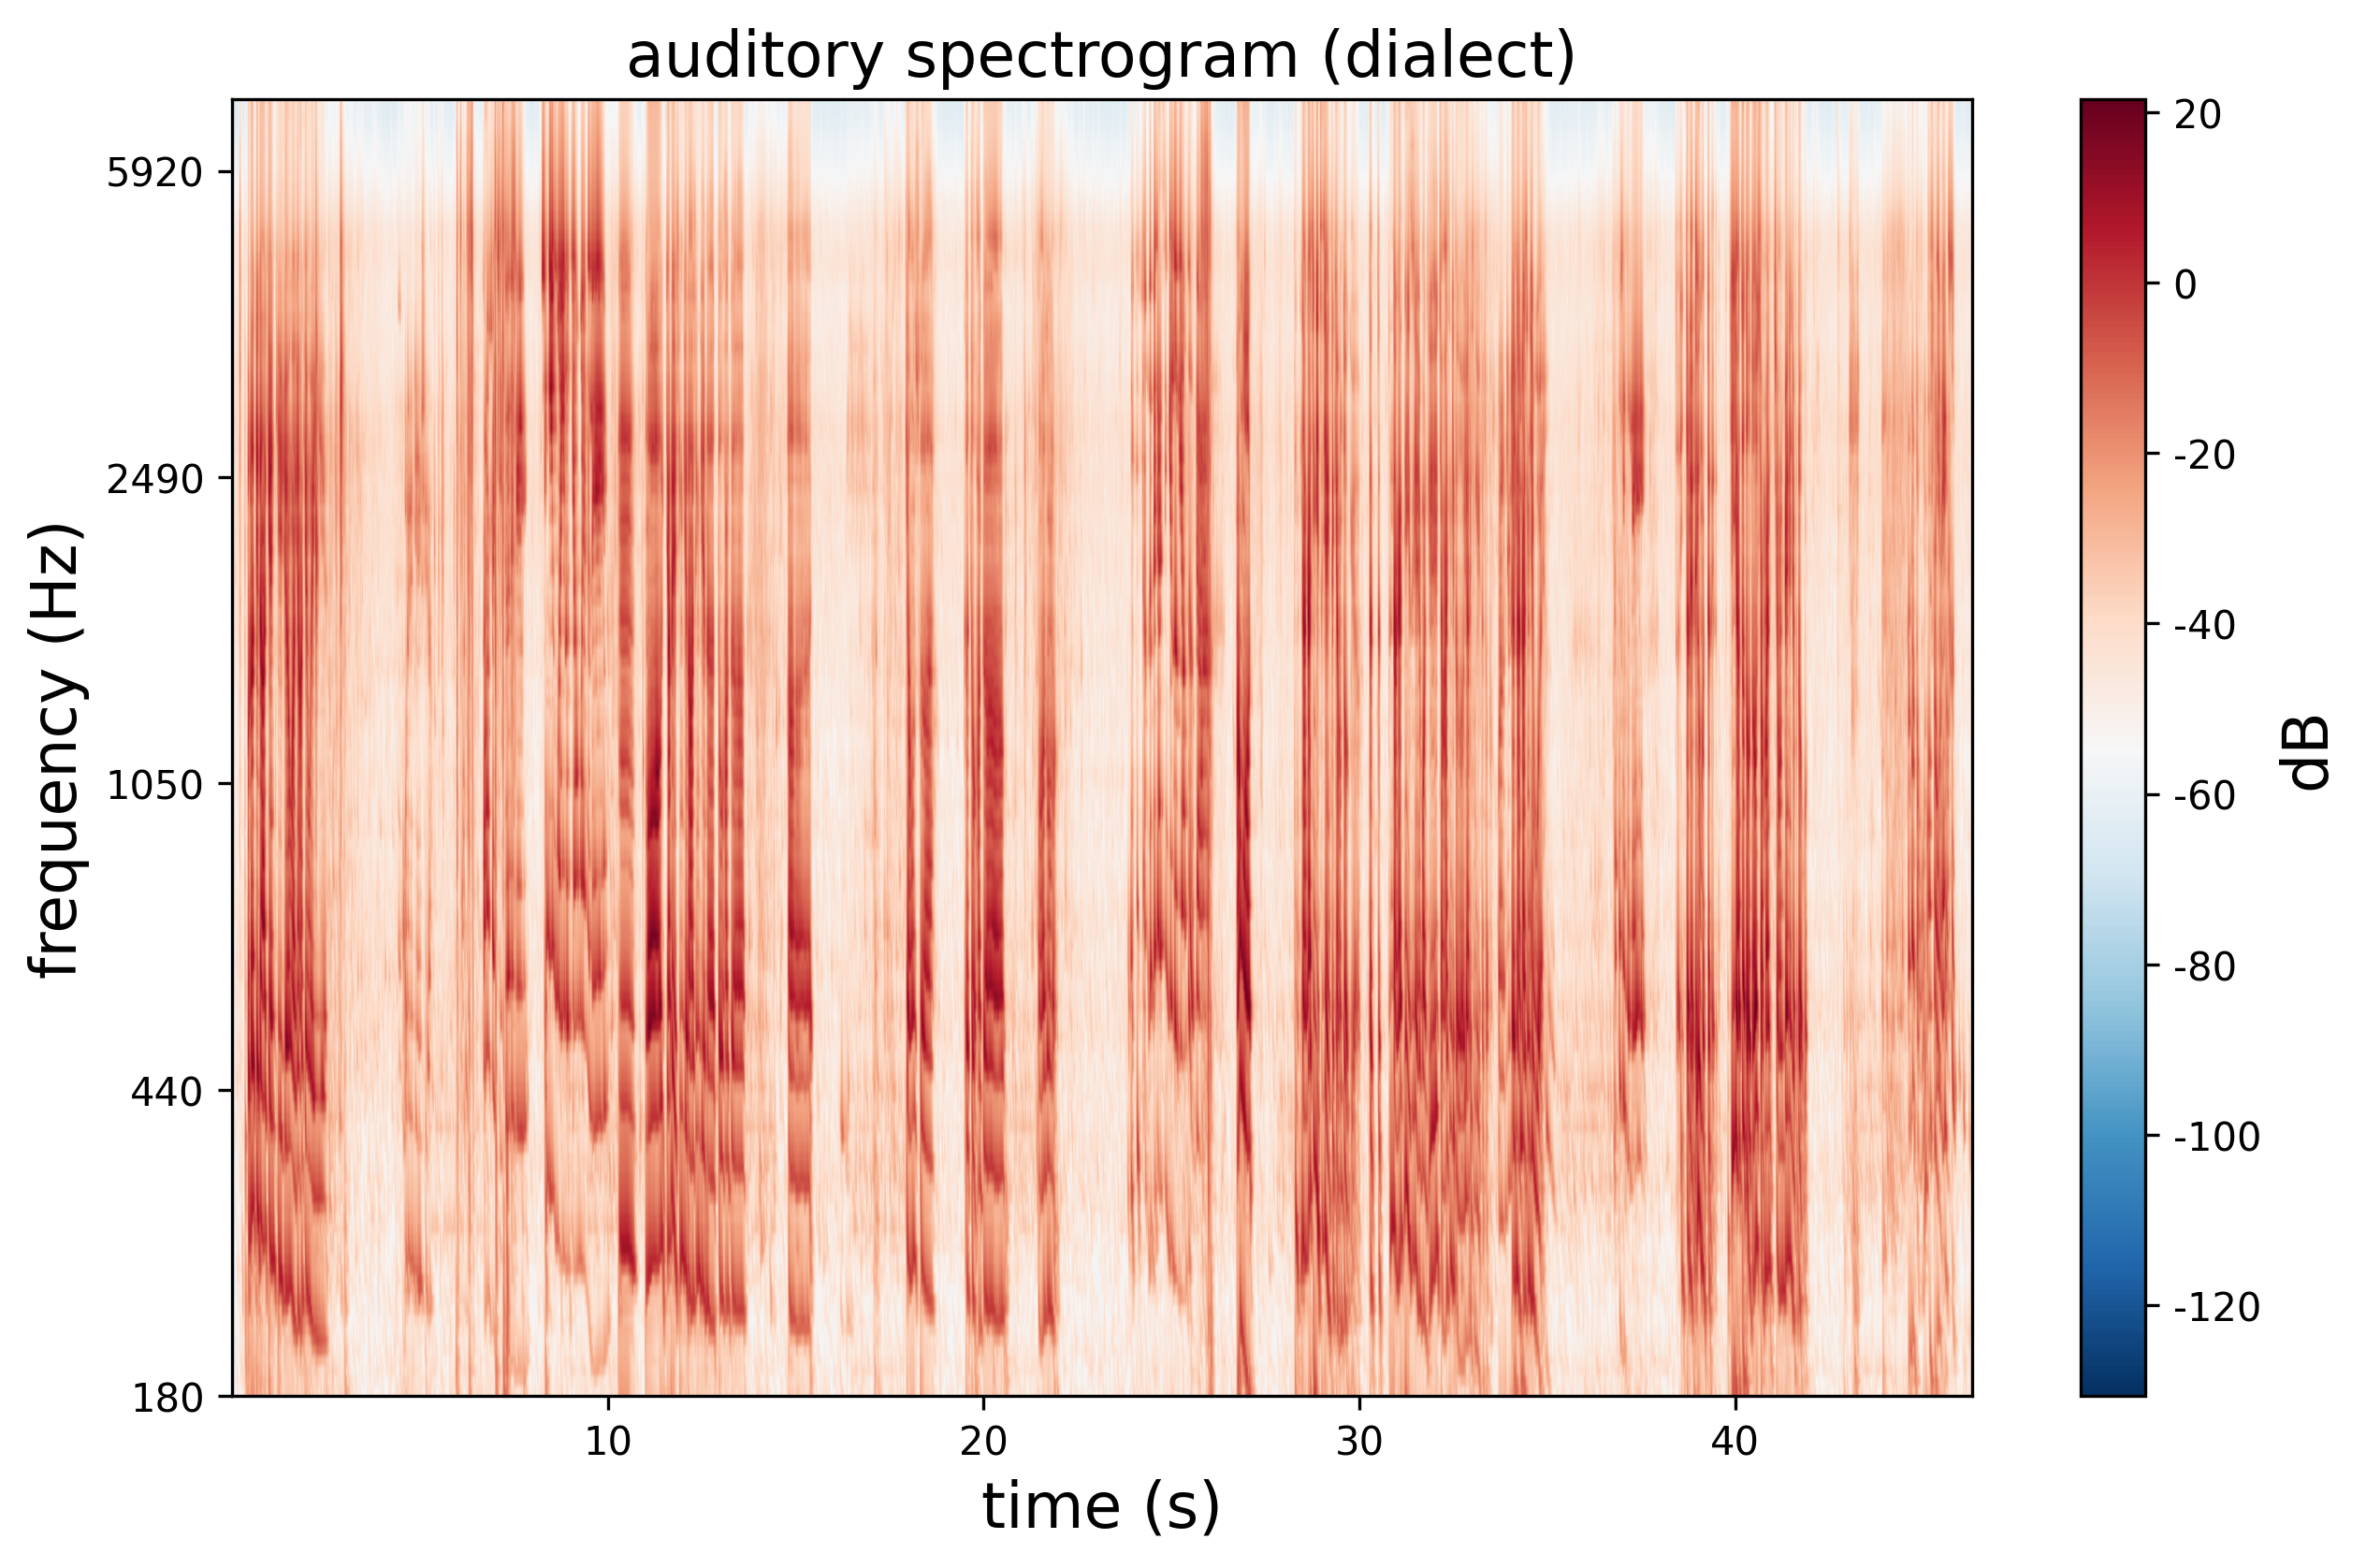
\includegraphics[width=\textwidth]{figure/dialect.png}
        \label{spectrogram:dialect}
    \end{minipage}
    
    \vspace{-2em} % 调整两行子图之间的间距
    
    % 第二行子图
    \begin{minipage}{0.49\textwidth}
        \centering
        \subcaption{}
        \vspace{-0.5em}
        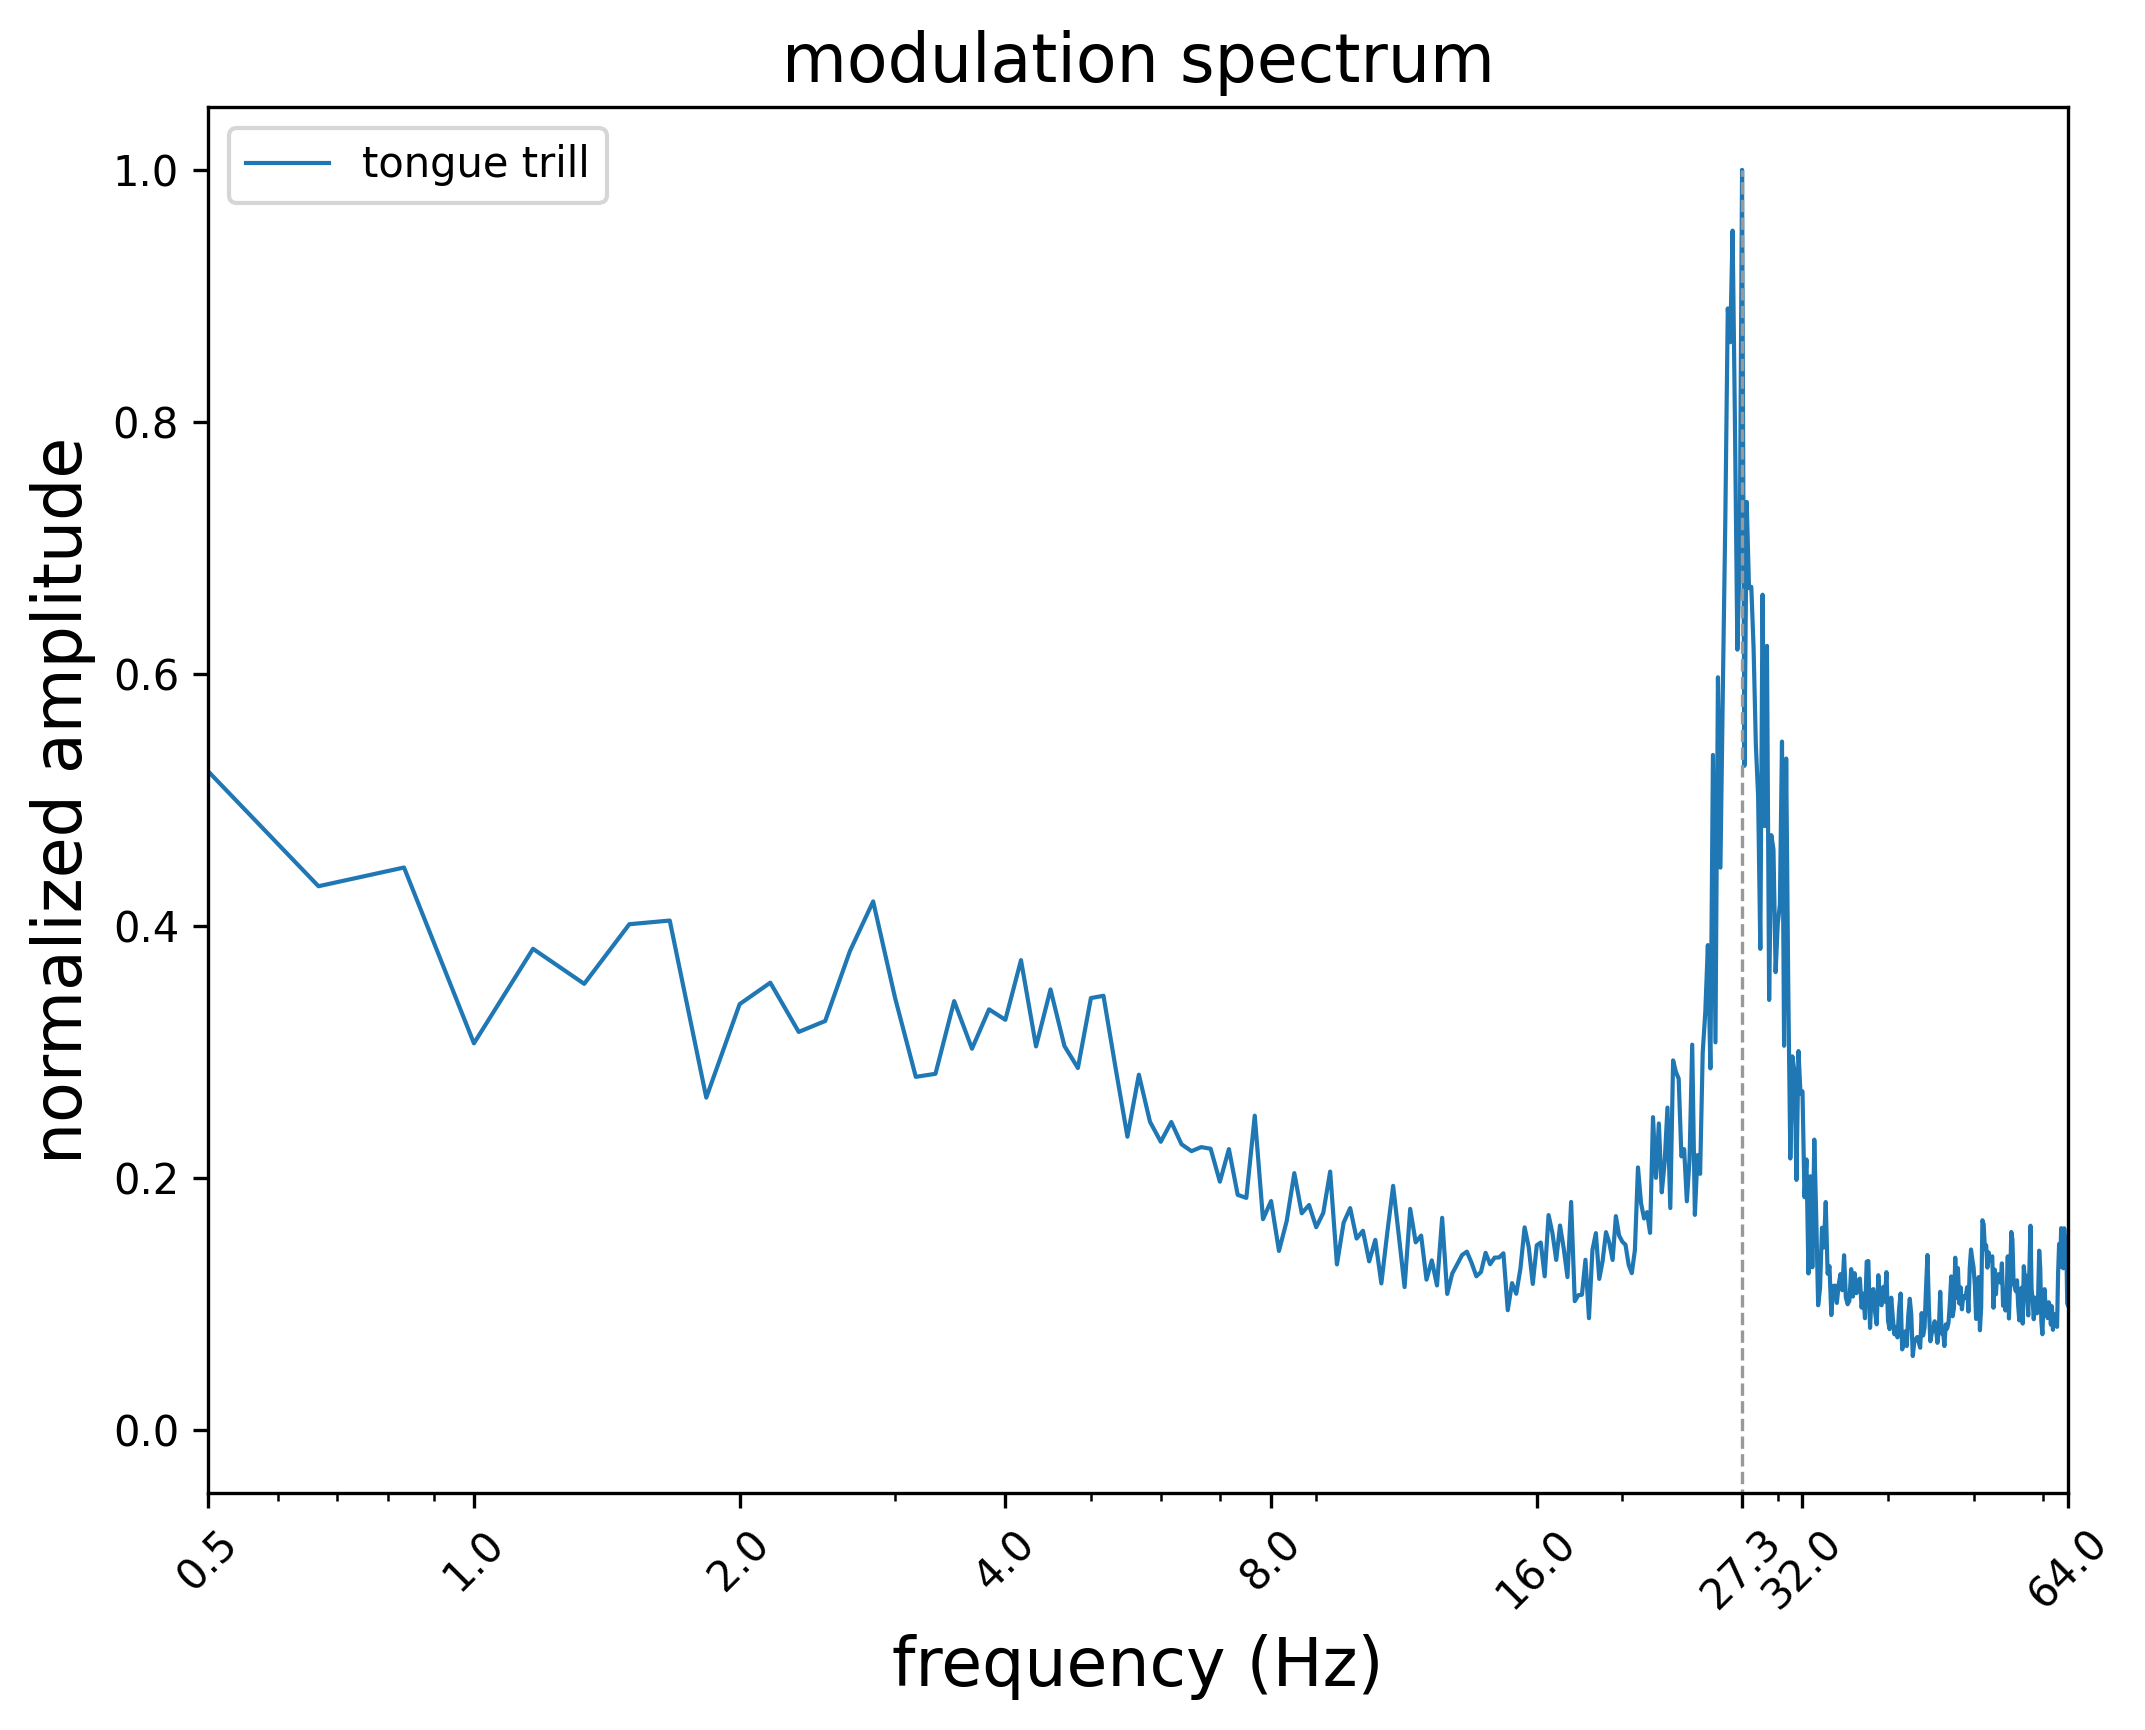
\includegraphics[width=\textwidth]{figure/spectrum_tanshe.png}
        \label{spectrum:tanshe}
    \end{minipage}
    \begin{minipage}{0.49\textwidth}
        \centering
        \subcaption{}
        \vspace{-0.5em}
        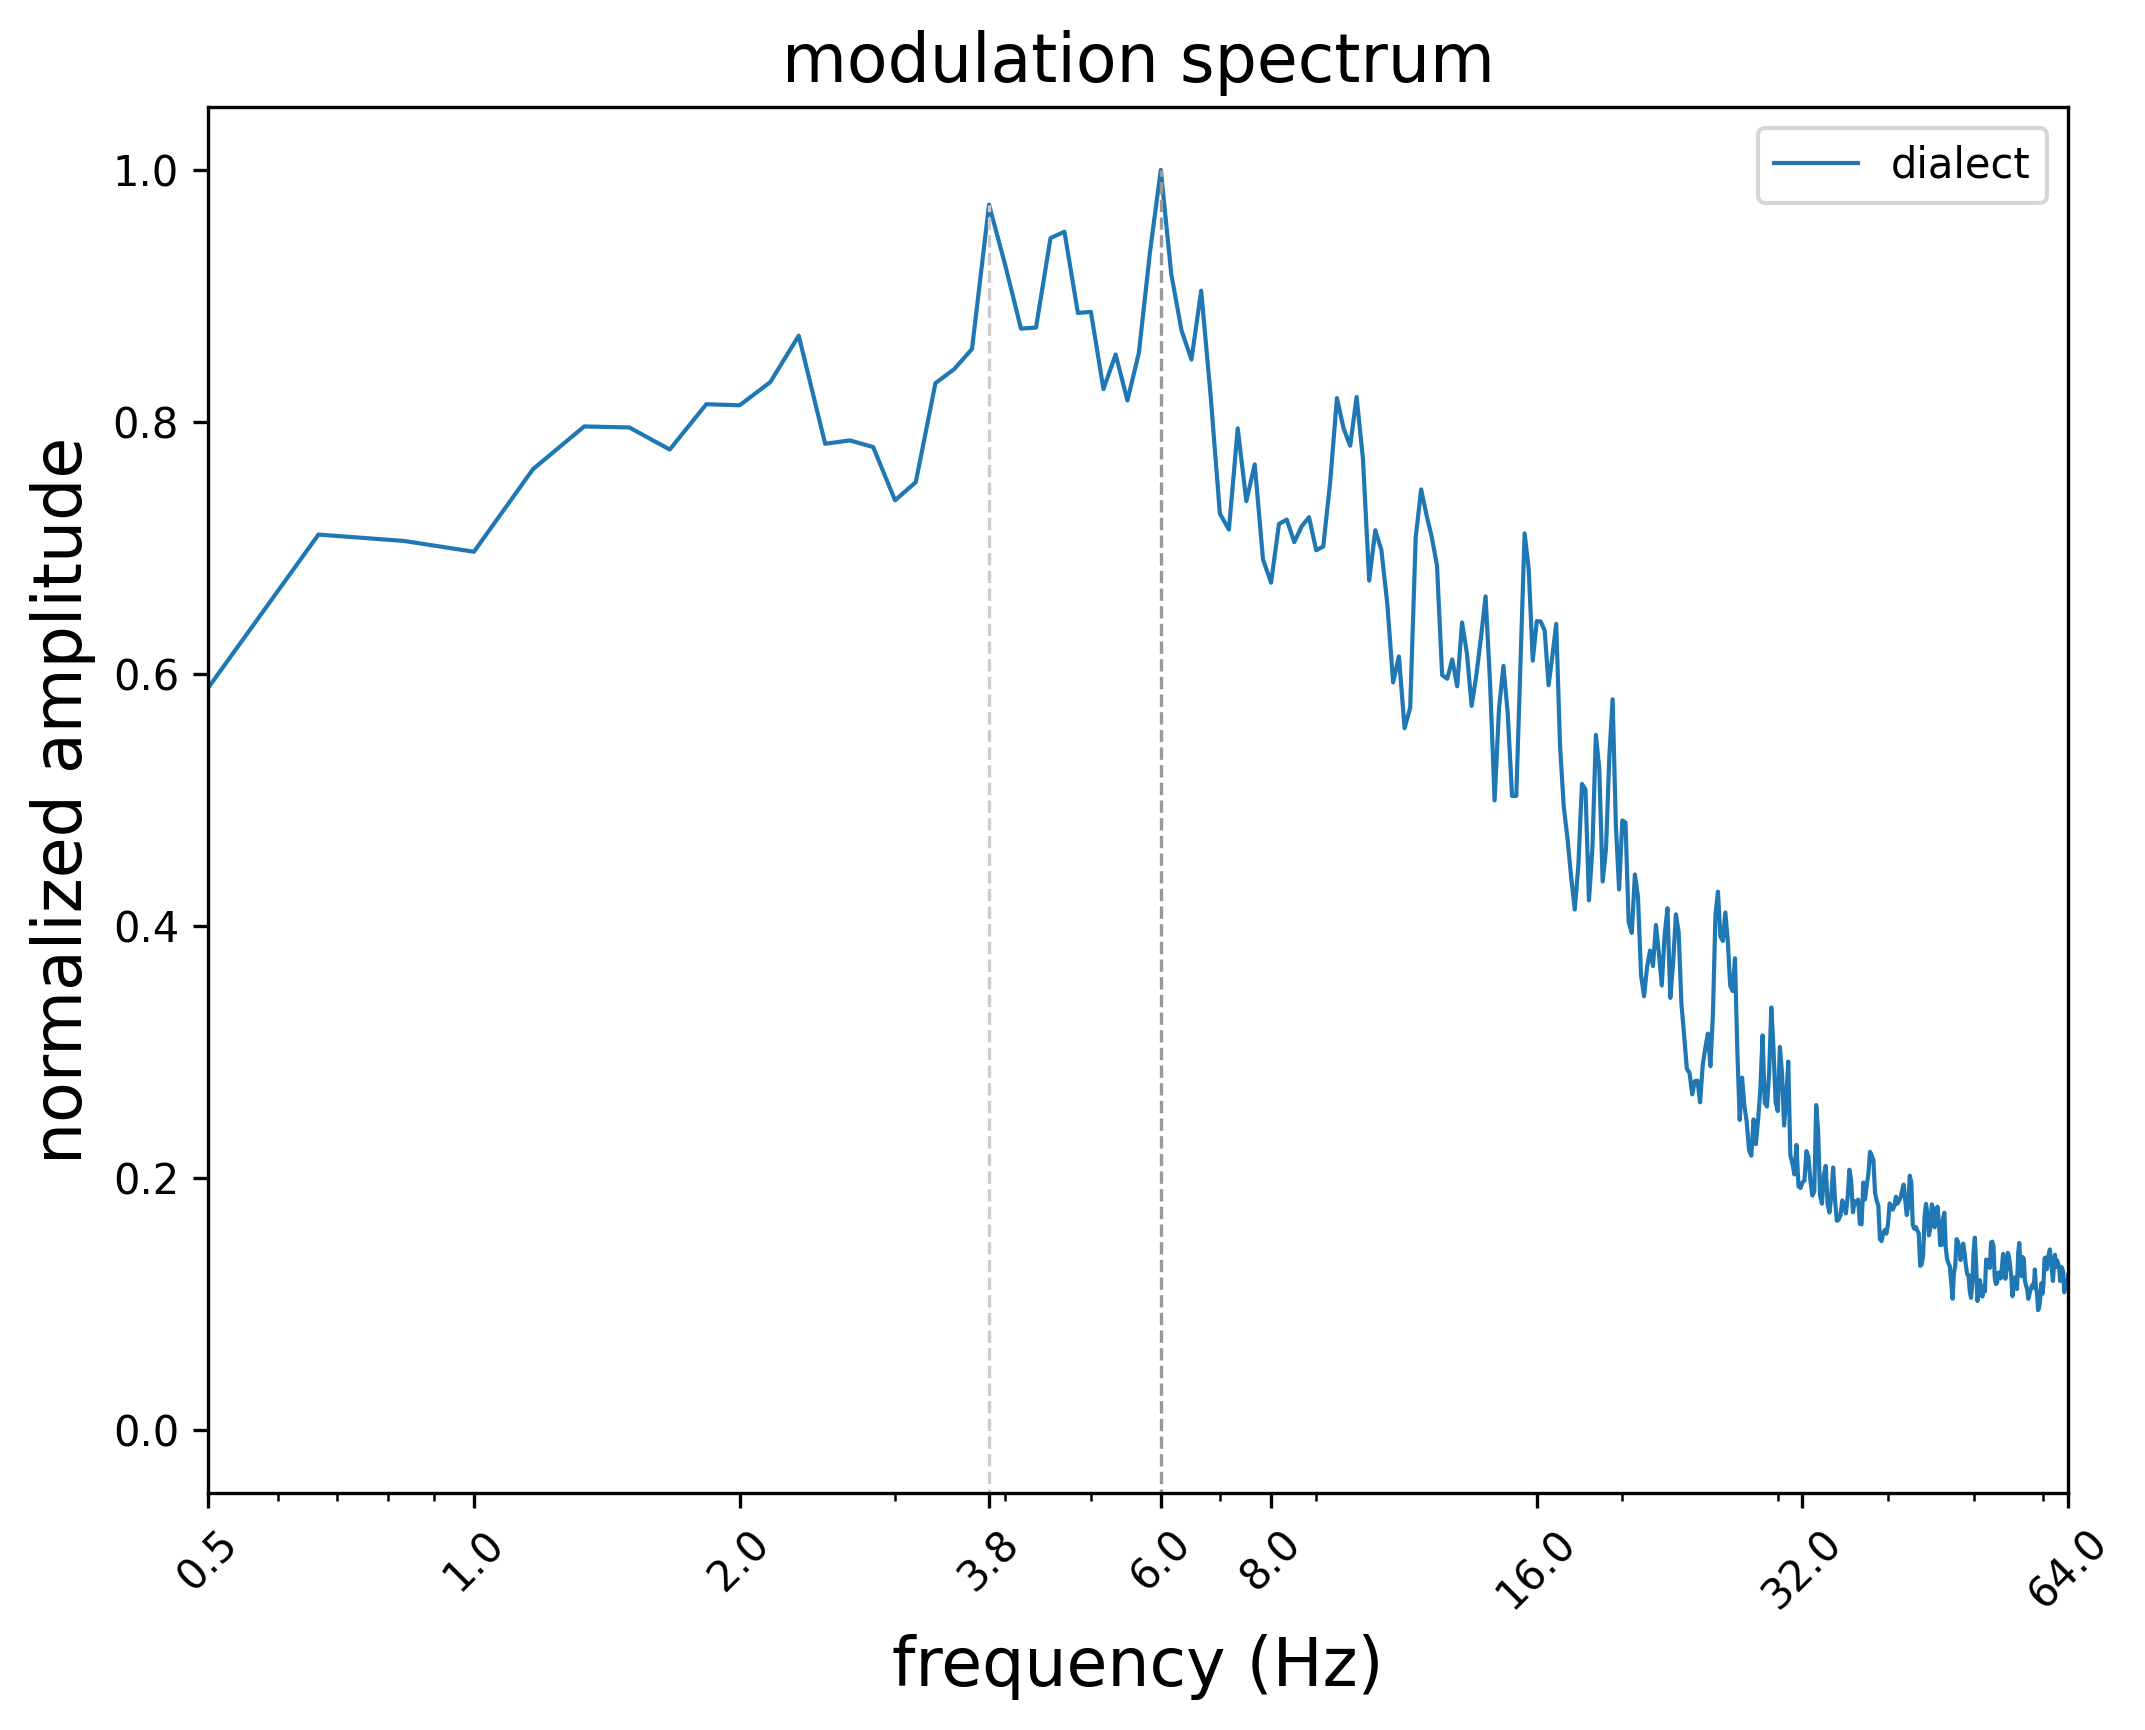
\includegraphics[width=\textwidth]{figure/spectrum_dialect.png}
        \label{spectrum:dialect}
    \end{minipage}
    
    \captionsetup{labelsep=period}
    \vspace{-1em}
    \caption{\small 弹舌和方言交流的时频图和调制谱}
    
    \label{fig:fig2}
\end{figure*}

\subsection{\heiti 身体运动产生的声音的调制谱分析}

弹舌产生的声音的时频图和调制谱分析见图\ref{spectrogram:tanshe}和\ref{spectrum:tanshe}。从调制谱图中可以看出,弹舌最主要的调制频率为27.3Hz的,且调制谱主要集中在这个频率。这个频率远高于正常人声的调制频率,因此我们可以推测存在齿龈颤音的语言的调制谱会在20-30Hz之间存在一个小波峰。然而,在\textcite{ding2017temporal}研究的9种语言中,法语、瑞典语、挪威语、荷兰语中都有齿龈颤音这种辅音,但是研究中得到的调制谱却没有20-30Hz之间的小波峰。这或许是因为这些语言中齿龈颤音的使用频率较低,因此在整个语音中的占比较小,不足以在调制谱中产生明显的效果。

不过,基于实验者自身的经验,俄语中弹舌的使用频率较高,因此实验者猜测在俄语的调制谱中可能会有一个20-30Hz之间的小波峰。为了验证该想法,实验者在某视频网站上找了一个的播客视频,视频内容为两个俄罗斯人在用俄语交流,时长为7分17秒。实验者对这段视频进行了调制谱分析,结果显示在20-30Hz之间并不存在一个小波峰,结果和之前研究中法语、瑞典语、挪威语、荷兰语的调制谱十分相似。这说明总体而言,齿龈颤音的使用并不会影响语言主要的调制频率。


\subsection{\heiti 方言调制谱分析}

实验者和家人使用方言交流的时频图和调制谱分析见图\ref{spectrogram:dialect}和\ref{spectrum:dialect}。从调制谱图中可以看出,实验者家乡的方言的调制谱在3.8Hz-6Hz之间有一个波峰,且6Hz为主要的调制频率。比较实验者阅读和方言的调制谱可以发现(见图\ref{fig:four}),实验者家乡方言的调制频率稍微快于实验者普通话阅读的调制频率,且方言调制谱的波峰会更宽。观察方言的时频图可以看出,实验者和家人用方言交流时句子短促,一般会在较短的时间内发出多个音节。这或许和中国南方方言没有翘舌音有关,翘舌音的存在可能会减慢字词的发声速率。

\begin{figure}[H]
    \centering
    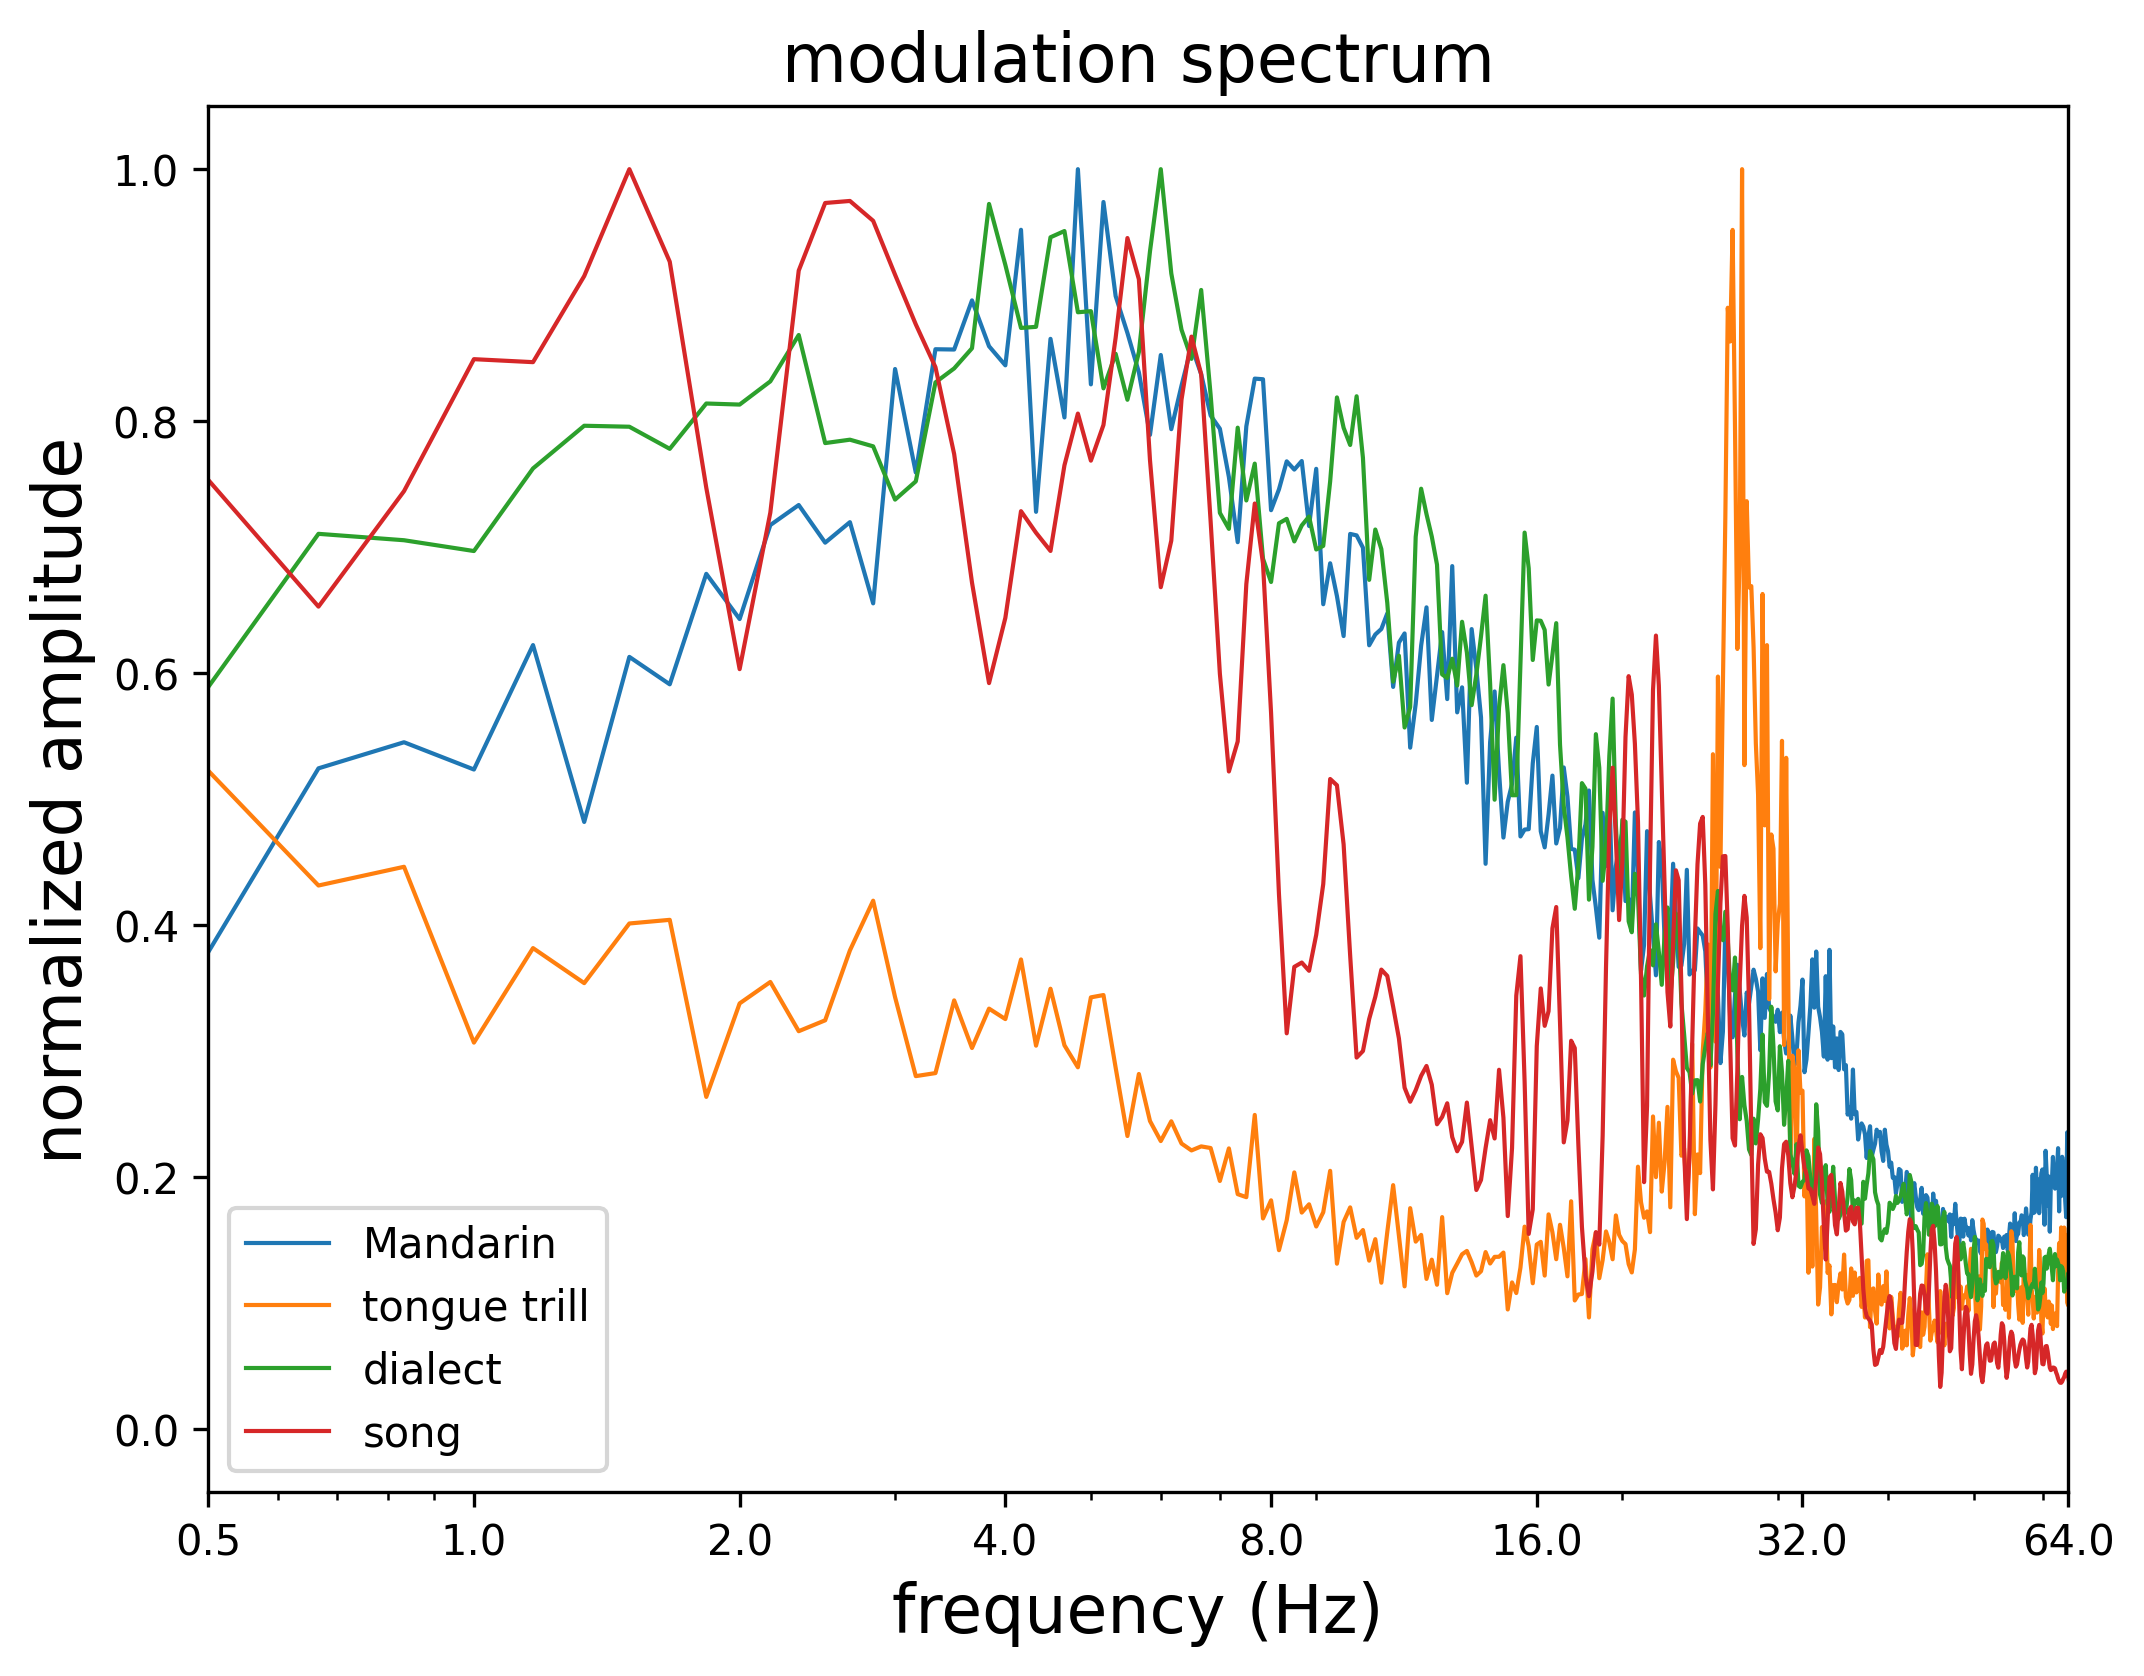
\includegraphics[width=\linewidth]{figure/spectrum_four.png}
    \captionsetup{labelsep=period}
    \caption{\small 语音、歌唱、弹舌和方言的调制谱对比}
    \label{fig:four}
\end{figure}


\section{讨论}

本实验旨在初步探讨个人语音、歌唱及身体动作的调制频率特性,并与\textcite{ding2017temporal}在大规模语料库上得出的关于语言和音乐调制分析进行比较。尽管本实验的样本量极为有限且仅基于个体数据,实验结果仍很大程度上支持了先前研究揭示的核心差异模式,同时也观察到了一些特定发声条件下的调制特征细节。

实验最重要的发现之一是验证了语音和音乐在慢速调制频域(主要指低于10Hz的范围)存在的显著差异。本实验中,普通话阅读样本的调制谱峰值出现在约4.8Hz,这与\textcite{ding2017temporal}发现的语音调制频率集中在4-5Hz范围(与平均音节速率相关)的结论高度一致。相对地,普通话歌唱样本的主调制峰值则位于约1.5Hz,显著低于语音峰值,且该频率非常接近于所演唱歌曲的理论节拍率(88bpm约等于1.467Hz)。此外,在歌唱调制谱中观察到的2.7Hz和5.5Hz附近的次级峰值,也大致对应于理论节拍率的整数倍(约2倍和4倍),这进一步印证了Ding等人(2017)关于音乐调制谱结构常与节拍及其谐波成分相关的发现。这些结果表明,即使在单一说话者/歌唱者的样本中,语音和音乐在基本声学节奏上的区分特征也是稳健存在的,反映了两者在产生机制和功能上或许占据不同的频域。

除了核心差异外,本实验也观察到了一些特定条件下的调制谱细节。方言交流样本的调制峰值(约6Hz)略高于普通话阅读,且波峰形态更宽,这可能反映了该特定方言或交流情境下较快的语速、较短的语句单元或独特的韵律模式。尤为引人注目的是弹舌(tongue trill)样本,其在约27.3Hz处展现出一个能量集中的调制峰值,清晰地反映了舌尖快速颤动这一发声动作的物理时间频率。然而,尽管齿龈颤音存在与较多语言中,但在这些语言的平均调制谱中并未出现类似的高频峰值。本实验的结果支持一种解释,即在自然语言流的整体平均分析中,特定音素(尤其是出现频率不高的音素)所具有的独特高频调制特征可能会被平滑或掩盖。此外,在歌唱样本的20-30Hz频段观察到的微弱波峰,与\textcite{ding2017temporal}研究中的中提琴的调制特性有相似之处,提示人声在歌唱时可能产生某些此前未被充分关注的高频调制成分,其具体来源(如声带振动模式、共鸣特性或特定发声技巧)有待进一步研究。

然而,本实验作为课程实验,仍存在显著的局限性。实验中所有数据源于单一实验者及有限的语音材料。因此,实验结果的普适性受到极大限制,主要价值在于作为一种初步的概念验证和对先前大规模研究发现的个体化印证。与此相对,\textcite{ding2017temporal}的研究是建立在涵盖多种语言和音乐风格、总时长达数十小时的大规模、多样化语料库基础之上,其结论具有更强的统计效力和普遍意义。

\printbibliography[title={\heiti 参\ 考\ 文\ 献}]

\end{document}

